\documentclass[a4paper,12pt]{article}
%\usepackage{t1enc}
\usepackage[longnamesfirst, round]{natbib}  % Bindet den natbib-standard fuer das Zitieren ein
%\usepackage{epsfig}
\usepackage[latin1]{inputenc}   % Ermoeglicht Sonderzeichen direkt einzugeben
\usepackage[T1]{fontenc}        % Garantiert saubere Worttrennung bei Umlauten etc.
\usepackage{color}              % Farbpaket
\usepackage[fleqn]{amsmath}
\usepackage{amsfonts,amssymb}   % ermoeglicht mathematische Sonderzeichen
%\usepackage{ngerman}           % neue deutsche Rechtschreibung
\usepackage[english]{babel}     %
\usepackage{ae}                 %
\usepackage{graphicx}           % Ermoeglicht das Einbinden von Bildern in allen Formaten
\usepackage{longtable}          % zum erstellen von Tabellen ber mehrere Seiten
\usepackage{multirow}           % zum Verbinden von Zeilen innerhalb einer Tabelle
\usepackage{pictexwd}           % PicTex, ein Graphikpaket
\usepackage{pst-all, multido}   % psTricks, ein Graphikpaket
\usepackage{url}
\usepackage[font=small,labelfont=bf]{caption}
\usepackage{amsmath} %for hats 
\usepackage{dcolumn}
\usepackage{amsthm}
\usepackage[font={footnotesize}]{caption}
\captionsetup[figure]{justification=raggedright,singlelinecheck=false}
\usepackage[super]{nth} %only for 1st 2nd 3rd etc
\usepackage{appendix}
\usepackage{dcolumn}
\usepackage{pdflscape}
\usepackage{booktabs}
\usepackage{threeparttable}
\usepackage{rotating}
\usepackage{hyperref}
\usepackage{setspace}
\usepackage{threeparttable}

% ________________ EINRICHTEN DES DOKUMENTS ______________________%

\bibliographystyle{plainnat}    % legt den Stil fuer das Inhaltsverzeichnis fest

\oddsidemargin 0.0in \evensidemargin 0.0in \textwidth 15.5cm \topmargin -0in \textheight 24.5cm \hoffset 0.00in
\parindent 0.7cm      % legt die Seitenraender fest

\pagestyle{plain}          % leere Kopfzeile, Seitennummer in der Mitte der Fusszeile

%\newcommand{\bs}{\boldsymbol}  % shortcut zur Erzeugung von fetten Sympolen in der Mathe-Umgebung

\renewcommand{\baselinestretch}{1.25}
% 1,5 -facher Zeilenabstand (Standard ist 1,2-facher Zeilenabstand, also 1,2*1,25 = 1,5

\usepackage{array, boldline, makecell, booktabs}

%\newcommand\btrule[1]{\specialrule{#1}{0pt}{0pt}}
%\usepackage[svgnames, table]{xcolor}

\begin{document}

% ________________ TITELSEITE ______________________%


\pagenumbering{roman}   % roemische Zahlen zur Seitennumerierung

\begin{titlepage}       % Umgebung fuer Titelseite, frei gestaltbar

\thispagestyle{empty}   % keine Numerierung auf Titelseite


\begin{center}
\vspace*{2.5cm}
{\bf  \Large   Economic Cost of Crime }\\
\vspace*{1cm} 
{\bf  \Large   Does Crime impact Economic Growth?}\\
\vspace*{3cm} 
Term Paper\\
Prof. Dr. Nora Markwalder and Dr. Monika Simmler
\\ Criminology Class\\

\vspace*{0.5cm} 
December \nth{20}, 2020\\
\end{center}

\vfill
\begin{flushright}
   \emph{Erik-Jan Senn} \\
    \emph{Langgasse 56}\\
    \emph{9008 St. Gallen}\\

\end{flushright}



% 
% \begin{center}
% $ $			% oeffnet und schliesst eine Matheumgebung (Trick, um den Titel nach unten zu rutschen
% \vspace{4cm}
% 
% {\LARGE TITEL}
% \vskip 4cm
% 
% Diese Seite ist frei gestaltbar
% \end{center}

\end{titlepage}

\newpage                % erzwingt an dieser Stelle einen Seitenumbruch


% ________________ Antiplagiatserklärung ______________________%


% ________________ INHALTSVERZEICHNIS ______________________%

% 


% ________________ HAUPTTEIL ______________________%



\pagenumbering{arabic}      % Seitenzahlen wieder arabisch numerieren
\setcounter{page}{1}        % Ruecksetzen des Seitenzahlzaehlers auf 1


\subsection*{\textit{Abstract}}

\textit{Abstract}


\section{Introduction}
\label{Introduction}
Economic cost of crime are any cost associated with the prevention or the consequences of criminal activities and is usually measured in monetary units.
Tangible economic cost of crime are measured in a monetary value already which makes them easy to estimate. They include direct cost such as repair cost for damaged goods, cost for medical care, cost for police and justice services and indirect cost such as prevention cost, loss of economic output (goods, services) or lost tax revenue.
Intangible economic cost of crime  need to be transformed into a monetary value and are harder to measure. Examples are pain caused by crime, reduces quality of live of victims, fear of persecution of the offender or reduced trust in strangers for the entire society (see Table \ref{tab:unit_cost_crime}).  \citep{kosten_nutzen_entorf} 

The first crime cost estimation method discussed in this paper tries to estimate each component of cost separately and then sums up the components.
This "detailed" estimation of crime cost could be used to evaluate justice policy using cost and benefit analysis. Take this simple question as an example: Is it profitable to introduce police patrols in cities at night? The question could be answered from an economic perspective if estimates for the following aspects are available: (1) cost for police patrols, (2) changes in prevented, detected and committed crimes due to police patrols and (3) economic cost of crime for each individual crime that is affected by police patrols. If that is the case, we could evaluate the question by comparing the cost of the measure (1) and the benefits of the measure (combine (2) and (3)).
However, apart from (1) which mainly consists of direct cost, it is hard to find sufficient data for estimate (2) and (3). Unit crime costing methods as described in Section \ref{Literature Review} estimate the cost of an individual crime as required for (3), but results show a high variation in cost and are mainly available for the US. 
Overall, the idea of using cost and benefit analysis for justice policy evaluation is often not feasible because especially intangible cost of crime are hard to measure.

The second crime cost estimation method does not attempt to capture each cost component separately (e.g. does not differentiate between tangible and intangible cost) and calculate a static cost estimate - it tries to estimate an effect of criminal activity on economic outcomes.
Specifically, the empirical analyses of this paper is based on the idea of \citep{entorf} and tests if crime rates negatively impact GDP-growth of countries in Europe.\footnote{Due to lack of sufficient data, the paper focuses on Europe and not on Switzerland.
Interestingly, in 2014 a request from the Christian Democratic Party (CVP) to the Swiss parliament asked to investigate the economic cost of crime in order to make more efficient investments in prevention and the justice system. The request was turned down due to the high cost to conduct the analysis.\citep{postulat}.}
Compared to the case specific analysis first method, this approach requires less data and could potentially capture more unobserved effects such as a change in victims risk tolerance or reduced trust in society due to crime.
Because economic outcome variables are also impacted by non-crime related factors, additional control variables need to be introduced and the effect measure is more noisy. 
Also, this more general analysis reduces the usability of the analysis for policy evaluation. A aggregated measure of crime such as case numbers or a crime index as usually used in this type of analysis is hard to directly influence by an institution. Justice system characteristics that are easier to impact such the share of prisoners or police expenditure would give a more direct interpretation and enhance the relevance of the analysis, but are unlikely have a measurable impact on economic outcomes. While static quantified effects in terms of overall economic variables are hard to interpret, the impact of crime on the dynamics of economic variables could be easier to grasp. \footnote{For example, it might be more interesting that criminal activity reduces the GDP by 0.5\% this year than to know that criminal activity accounts for 3 \% of the GDP.} 

The paper is organized as follows: Section \ref{Literature Review} gives an overview of the existing literature for crime-costing methods and macro analysis approaches. Section \ref{Methodology} introduces the empirical methods for this paper, Section \ref{Data} the data used. Section \ref{Results} presents the empirical results and Section \ref{Conclusion} concludes. 
\begin{table}
\begin{minipage}{0.9\textwidth}
\captionof{table}{Cost of Crime - Classification}
  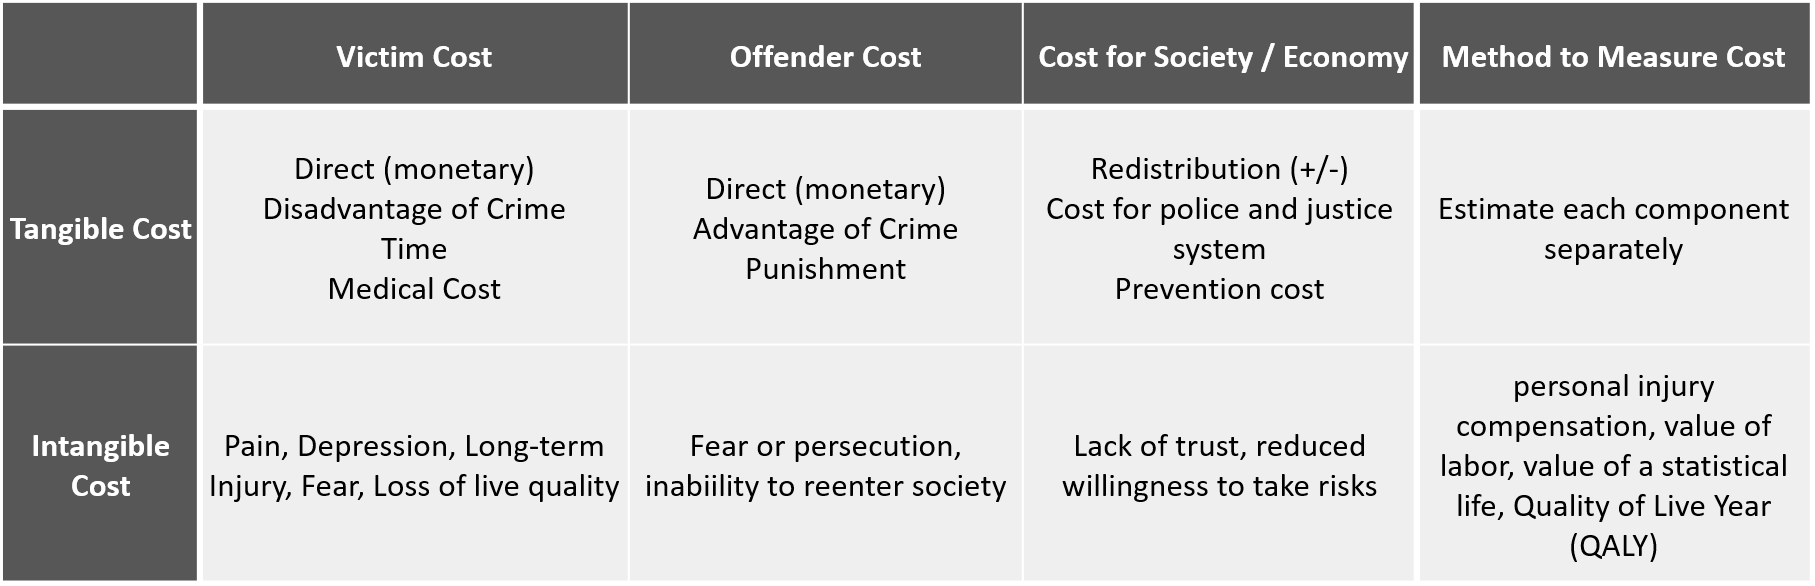
\includegraphics[trim={0 0 0 0},width=\linewidth]{charts/table_unit_cost.png}
\begin{flushleft}
\footnotesize{\textit{Note:} The table shows examples of cost of crime components classified in different categories and potential ways to measure the components separately. Source: own representation.
\label{tab:unit_cost_crime}	
}
\end{flushleft}
\end{minipage}
\end{table}


\section{Literature review}
\label{Literature Review}
The literature can be broadly divided into the two estimation methods discussed: the data-reliant detailed crime-costing methods that calculate cost of individual components and the less data-reliant macro perspective approaches. 


\subsection{Unit Crime Costing}
First, for crime-costing methods, I focus on research that includes intangible cost. Most estimations in the literature are based on US-data due easier access to detailed tangible cost data and similar availability of victim surveys etc..
To estimate intangible cost, various different approaches are used. 

The idea of a statistical value of a life (SVL) assigns a monetary value to a life e.g. by discounting the expected economic value generated by one person to the current date. It can be interpreted as the economic loss of death. \cite{viscusi} estimates the SVL to be 2 million USD.
The "jury compensation approach" by \citep{cohen1988} uses the SVL and historical risk of death for different crime categories to estimate intangible unit crime cost. However, this approach does not take other consequences such as disabilities or psychological issues into account.

Cost-of-illness approaches distinguish between different types of injuries. For example, determined monetary payments for injuries from health insurance or personal injury compensation payments determined by court could be used to value economic cost for the victim more accurately. 
The Quality-Adjusted-Life-Year (QALY) measure used in the health care sector is a numeric indicator between 0 and 1 that makes different health issues comparable. The willingness-to-pay to prevent a reduction in QALY can be estimated using surveys \citep{entorf}.
Similarly, the willingness-to-pay approach of \citep{cohen2004} values a crime by asking how much someone is willing to pay to reduce the chance of becoming a victim.\footnote{For example, if someone is willing to pay 100 USD to reduce the change of robbery by 10 \% , the estimated cost per case is 1,000 USD.} 
While all of these approaches mentioned might include most considerations of potential victims and offenders regarding a crime, they might not fully reflect intangible cost society such as mistrust or reduces willingness to take risks.

\cite{collister} show a summary of unit-cost of crime study results with different methods (see Table \ref{tab:unit_cost_crime_lit_review}). 
The type of offense has a large impact on the cost of crime estimates: estimates for violent crimes are higher than for property crimes, mostly due to medical cost, justice system cost and intangible cost. Murder has the highest estimated cost for every study, which can be explained by the economic loss of a life and high tangible cost of a homicide. 
Also, the unit cost estimates show strong variation across studies - the cost of robbery estimate for example lies between 18,591 USD and 280,237 USD. 

It is possible to use unit cost estimates to estimate the aggregated cost of crime by combining it with the case numbers. However, economically it could more plausible to see the cost estimates as marginal cost because cost per case might change with more or less cases due to economies of scale for the justice system or a potential critical threshold of crime that could lead to an economic breakdown. Common estimates are that economic cost of crime accounts for 3\% to 7\% of GDP for developed countries \citep{kosten_nutzen_entorf}.

\begin{table}
\begin{minipage}{0.9\textwidth}
\captionof{table}{Unit Cost of Crime}
  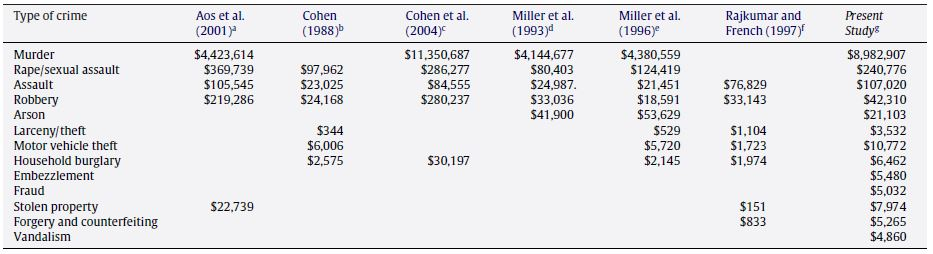
\includegraphics[trim={0 0 0 0},width=\linewidth]{charts/tab_lit_review.jpg}
\begin{flushleft}
\footnotesize{\textit{Note:} This table from \cite{collister} shows a summary of unit cost of crime estimates in the literature for different types of crimes. Source: \cite{collister}.
\label{tab:unit_cost_crime_lit_review}	
}
\end{flushleft}
\end{minipage}
\end{table}

\subsection{Macro Perspective}
The second approach discussed in this paper does not estimate a static cost of crime based on separate cost estimations, but interprets "cost" more broadly as the effect of crime on economic variables. 

Researchers use times series data of socio-economic indicators and crime measures of multiple regions. All papers presented here use a more or less sophisticated version of an auto-regressive (AR) model: the basic idea of an AR model is that past observations of the dependent help to explain future ones. 
Each effect estimation in this section consists of, firstly, an economic outcome variable such as GDP-growth, unemployment or house prices as dependent variable, secondly, one or multiple measures of crime such as case data for categories of crime or a crime index and, thirdly, a set of control variables that explains variation in economic outcomes that do are not connected to crime. 
A key challenge is to model the economic factor well enough to make a potential effect measurable because many other factors will have a stronger impact than crime.

The main model for the empirical section of this paper stems from \cite{entorf} and uses an AR(1) model for GDP-growth controlling for investment without fixed effects. They do not find a significant effect of crime on GDP-growth for European countries. With more detailed regional data, they find few significant effects. I would however question whether these are true significant effects or they are simply significant by change (\% significance level).
In Section \ref{Methodology}, \cite{entorf} sparse model will be adapted to control for more variables, and a different crime measure with a new notion of a causal effect will be introduced.
\cite{detotto} use the same idea with a more flexible model specification allowing for more long run effects using Italian crime data.

\cite{var_model} use a even more flexible vector-auto-regressive model to model the relationship between homicide rate shocks and the economic variables GDP-growth and foreign direct investment. In their VAR-model (the general case of an AR-model), multiple dependent variables are explained simultaneously and can impact each other. Their analysis using data from 32 Mexican states accounts for reverse causality (GDP-growth affects crime) and unknown time delay of effects and finds a GDP-growth reduction of 0.25\% after a shock of homicide rates.

\cite{columbia} investigate whether crime in Columbia had a significant effect on economic growth. Similar to the studies above, they use a cross section of economic indicators including education for all countries worldwide to explain log GDP per capita. They tackle reverse causality issues using instrumental variables for human capital and institutional power. However, they do not directly observe a crime measure, but simply include a dummy for Columbia and claim this is a measure of criminal activity. This seems to be a simplified measure of crime because the Columnbia dummy variable can also include other systematic differences in economic dynamics. 



\section{Methodology}
\label{Methodology}
Similar to \cite{entorf}, I want to measure cost of crime by the causal effect of changes in criminal activity on the change in GDP-growth. The hypothesis of a negative effect of crime on GDP-growth will be tested on a country level.
The aim is not to estimate the effect of crime for specific countries other values of some control variables (conditional average treatment effect), but an overall average treatment effect for countries in Europe.

\subsection{Causal Effects}
The causal effect idea used by \cite{entorf} states that if a variable helps to predict future values of another variable, this is a causal effect (Granger causality). The main part of this analysis uses a stronger notion of causality, called Rubin causality. A potential outcome is defined as the outcome that would occur if the variable of interest (treatment) takes a certain value. 
A Rubin causal effect is the difference in potential outcome for different values of the variable of interest (treatment). 
Importantly, only one potential outcome can be observed at a time, while other potential outcomes are called counter-factual. The main challenge to identify Rubin causal effects is to find a convincing empirical strategy to identify these counter-factual. 
The main framework for Rubin causality is easiest to apply to one binary treatment variable, therefore I will follow this approach.

The best empirical strategy to identify a Rubin causal effect of a treatment variable(s) (here crime measures) on some outcome (here real GDP-growth) is an experiment where treatment is randomly assigned to observations. However, as we cannot randomly assign criminal activity levels to countries, we need to control for systematic differences between areas with higher and lower criminal activity. 
Every variable that impacts both treatment and outcome needs to be included in a model to identify a causal effect (conditional independence). These variables are also called confounders.
We cannot have a causal effect of GDP-growth on regressors that are used to explain GDP-growth (no reverse causality). 

\subsection{Model}

I use a panel data regression to model country real GDP-growth. 
Real GDP-growth as an outcome variable brings the advantage that intangible effects of crime that are hard to capture separately are included in the measure. \footnote{It should be noted that by definition, GDP does not include economic value added from illegal activities which could lead to an downwards biased effect as higher crime would reduce legal economic output while total economic output would stay the same. }

\begin{equation}
\label{reg}
gdp_t = \beta X_t+ \alpha A_{t-1} + \eta B_t + \phi FI  + u_t
\end{equation}
Specifically, I estimate coefficients of the regression equation (\ref{reg}) above with $gdp_t$ denoting real GDP growth in time period t, $X_t$ denoting the crime measure(s), $A_{t-1}$ denoting lagged control variables, $B_t$ denoting leading control variables and $FI$ denoting time and country fixed effects. 

$X_t$ can include one or multiple crime measures (for the construction see next paragraph). For one binary crime measure, it equals the estimated average causal effect in the Rubin framework.   $A_{t-1}$ includes GDP itself (AR(1)), inflation, the ratio of total investment to GDP and the share of people with income below the poverty line \footnote{The risk-of-poverty (poverty line) threshold used is 60\% of the median disposable income.}. The measures are lagged to reduce the reverse causality which is highly likely (and GDP of course cannot be included without a lag). $B_t$ includes the share of the population with finished tertiary and secondary education and the share of young males \footnote{Young males are likely to systematically differ from other population groups in economic and criminal activity.}. The time fixed effects in $FI$ capture e.g. overall economic trends such as the financial crisis, but would also remove effects of common trends in crime development. Country fixed effects in $FI$ e.g. control for heterogeneity in the data generation of crime case numbers: crime detection rates, definitions of crimes or methods of counting cases could differ across countries.
Overall, this empirical model controls for few potentially revelant sources of variation in GDP-growth, and mainly relies on fixed effects to control for systematic differences between countries. While the main model purpose is not to model economic development, variation of GDP-growth should be partly explained by the model to decrease the variance of the effect estimate. The model does not account for potential delayed effects of crime. A causal effect of GDP-growth on crime could is plausible is not accounted for in the model.

\subsection{Measures for crime}
To measure criminal activity $X_t$, as in \cite{entorf}, police report case numbers for 7 offense categories (intentional homicide, assault, sexual violence, robbery, burglary, theft, drug crimes) are used. While \cite{entorf} make separate regressions for each offense type, this could violate the conditional independence assumption since a potentially relevant other crime variable is not included in the model. Therefore, I include all offense categories in one regression and test for joint significance of the coefficients.

For the Rubin-causal effect, I need a single binary crime index that classifies criminal activity as either high or low. The causal effect is then the change in outcome if crime would be high compared to low.

To construct such a crime index, my main idea is to compress as much information as possible of the 7 case numbers for offense categories into a single binary measure. 
Principal component analysis (PCA) is used to reduce the dimensions of the data (here to 1) while still explaining as much variation as possible. Principal components cannot be interpreted directly. The main assumption is that the first principal component contains most of the variation in general criminal activity while others contain more characteristics of specific crimes (see Section \ref{Data} and Table \ref{fig:princial_component_1} for evidence).
A simpler way to construct such an index could have been to assign a fixed weight to each offense category and calculate an aggregate index. 

The single continuous crime index is then converted into the "binary crime" measure (above mean of the continous crime index corresponds to high crime, below mean corresponds to low crime). Practically, this binary crime index constructed from case data of systematically different regions will often be constant over time because a region will always be above or below the average first principal component. In this empirical strategy with country fixed-effects, time variation in crime is needed to distinguish the effect from fixed-effects. Therefore, I also calculate the "binary crime country" index, which is set to high if crime is above the average for that specific country over the entire time frame. 

In total, I use 2 binary measures (binary crime, binary crime country), 2 continuous measures (principal component 1 and principal component 2) and all raw case numbers for different offense categories as crime measures. The preferred measure "binary crime country" most convincingly fulfills the conditional independence assumption in the given panel data model, but is also the most noisy one due to the loss of information when constructing the measure.  

\section{Data and Descriptives}
\label{Data}
I use socio-economic data and criminal record data from \cite{eurostat} for 32 European countries including Switzerland from 2009 to 2019. 
Police-reported case numbers per 100.000 inhabitants for 13 offense categories are reported for each country. I focus on 7 categories\footnote{Other categories are excluded because they are subcategories or have many missing datapoints.}: intentional homicide, assault, sexual violence, robbery, burglary, theft and drug crimes. 
Regarding missing data, I require all 7 crime measures and GDP-growth to be reported, otherwise an observation is excluded. For other control variables, I replace missing observations with the country mean. If a variable is missing for all years, the effect is already incorporated in the fixed effect of the country.
From 2008, crime records are only available on a country level and not on a regional level as before. Combined with a short time horizon and missing data, this leads to only 269 observations available for the analysis.

Table \ref{fig:princial_component_1} shows the factor loadings of the first and second principal component. All loadings apart from homicide for the first component are positive. The assumption that the first principal component reflects general activity well is questionable due to the different sign of homicide. Countries with more intentional homicides would have a lower crime index if case numbers of other offense categories do not change. The reduction of dimensionality can be see in Figure \ref{fig:crime_case_data} and Figure \ref{fig:princial_component_1}. While general crime trends seem to be captured by the index, fixed positive weights or an already existing crime index could have prevented the negative impact of homicide on the crime index. If murder rates do not vary too much across time in one country, this should not be a big issue because the analysis does not focus on a cross-sectional comparison of countries. \footnote{A more detailed comparison with already existing crime incides is necessary to verify the validity of this measure.}
The low variation of the crime index for many countries in Figure \ref{fig:princial_component_1} might be an issue for the empirical analysis because a less marginal difference from high to low criminal activity makes estimation of a potential effect harder. 


\begin{singlespace}
		\begin{table}[!htbp]
			\centering
			\def\sym#1{\ifmmode^{#1}\else\(^{#1}\)\fi}
			\begin{threeparttable}
				\caption{Crime Measure - Principal Component Factor Loadings}\label{pca_factor_loadings} 
\begin{tabular}{rrrrrrrr}
  \hline
 & PC crime 1 & PC crime 2 \\ 
  \hline
intentional homicide & -0.23 & 0.22 \\ 
  assault & 0.27 & 0.60 \\ 
  sexual violence & 0.46 & -0.08  \\ 
  robbery & 0.27 & 0.63 \\ 
  burglary & 0.47 & -0.04\\ 
  theft & 0.50 & -0.15  \\ 
  drugs & 0.35 & -0.41 \\ 
   \hline
\end{tabular}
\begin{footnotesize}
				\begin{tablenotes}
					\item \textit{Note:} This table shows the factor loadings of the case numbers of different offense categories for the constructed crime measures. A factor loading can be interpreted as the weight of a variable within the principal component. PC 3-7 are ommitted as they are never used for the analysis. Most importantly for this analysis, the first principal component weights all have the same sign apart from homicide. This component and the binary transformation is used as the main crime index measure in this analysis.\\ 
				\end{tablenotes}
			\end{footnotesize}
			\end{threeparttable}
\end{table} 
\end{singlespace}

Table \ref{tab:descriptive_stats} shows descriptive statistics for the 269 observations\footnote{\cite{entorf} use 62 observations.}. The last two columns show subpopulation means for all observations with a high/low crime level according to the "binary crime country" measure. GDP-growth is 1.4 \% lower in times of higher criminal activity than in times of lower criminal activity within a country, also some other control variable means differ depending on crime.\footnote{A test could be conducted to test if the difference in means is statistically significant.} The group means for the raw crime data of sexual violence and drugs are lower for observations with higher crime level even though they positively influence the continuous crime index. This is possible because of the separate construction of crime measures by country and correlations between case numbers of different offense types.


% latex table generated in R 3.6.1 by xtable 1.8-4 package
% Sun Dec 20 01:43:42 2020
\begin{singlespace}
		\begin{table}[!htbp]
			\centering
			\def\sym#1{\ifmmode^{#1}\else\(^{#1}\)\fi}
			\begin{threeparttable}
				\caption{Descriptive Statistics}\label{tab:descriptive_stats} 
\begin{tabular}{rrrrrr}
  \hline
 & Mean & Median & St.-Dev. & Mean - Low Crime & Mean - High Crime \\ 
  \hline
    gdp & 1.54 & 1.90 & 3.37 & 2.20 & 0.80 \\ 
    \hline
intentional homicide & 1.34 & 1.08 & 0.95 & 1.40 & 1.26 \\ 
  assault & 78.98 & 35.72 & 131.50 & 73.69 & 84.89 \\ 
  sexual violence & 35.18 & 20.86 & 39.67 & 35.82 & 34.47 \\ 
  robbery & 57.52 & 40.33 & 52.51 & 51.86 & 63.84 \\ 
  burglary & 470.35 & 405.83 & 316.39 & 411.65 & 535.99 \\ 
  theft & 1379.72 & 1200.28 & 1145.97 & 1240.69 & 1535.18 \\ 
  drugs & 248.48 & 93.99 & 300.52 & 251.59 & 245.01 \\ 
    \hline
  gdp lag1 & 1.41 & 1.80 & 3.39 & 2.00 & 0.74 \\ 
  inflation lag1 & 97.03 & 99.10 & 5.16 & 97.64 & 96.34 \\ 
  investment lag1 & 21.23 & 21.21 & 3.72 & 20.87 & 21.62 \\ 
  poverty lag1 & 24.68 & 21.20 & 8.66 & 24.61 & 24.76 \\ 
  educ university & 38.53 & 40.70 & 9.99 & 39.80 & 37.12 \\ 
  educ secondary & 77.53 & 80.70 & 13.12 & 78.87 & 76.03 \\ 
  young males & 17.44 & 17.40 & 1.09 & 17.24 & 17.66 \\ 
   \hline
\end{tabular}
\begin{footnotesize}
				\begin{tablenotes}
					\item \textit{Note:} This table shows descriptive statistics for the entire sample and for the observations classified as low and high crime (by the binary crime per country measure). Differences in means between high and low crime could indicate a systematic difference between both groups which makes the variable a potential candidate for the analysis.\\ 
				\end{tablenotes}
			\end{footnotesize}
			\end{threeparttable}
\end{table} 
\end{singlespace}


In Figure \ref{fig:corr_matrix_paper}, correlations of the main variables of interest are investigated. From the 4 constructed crime measures, only "binary crime country" is slightly negatively correlated with GDP-growth. Education and young males are correlated with crime measures and GDP-growth, indicating that they need to be included in the analysis to not violate the conditional independence assumption. Lagged GDP-growth and inflation could be useful covariates to reduce the variance of the estimation due to their strong correlation with GDP-growth. 

\begin{figure}
\begin{minipage}{0.9\textwidth}
\captionof{figure}{Correlation Matrix}
  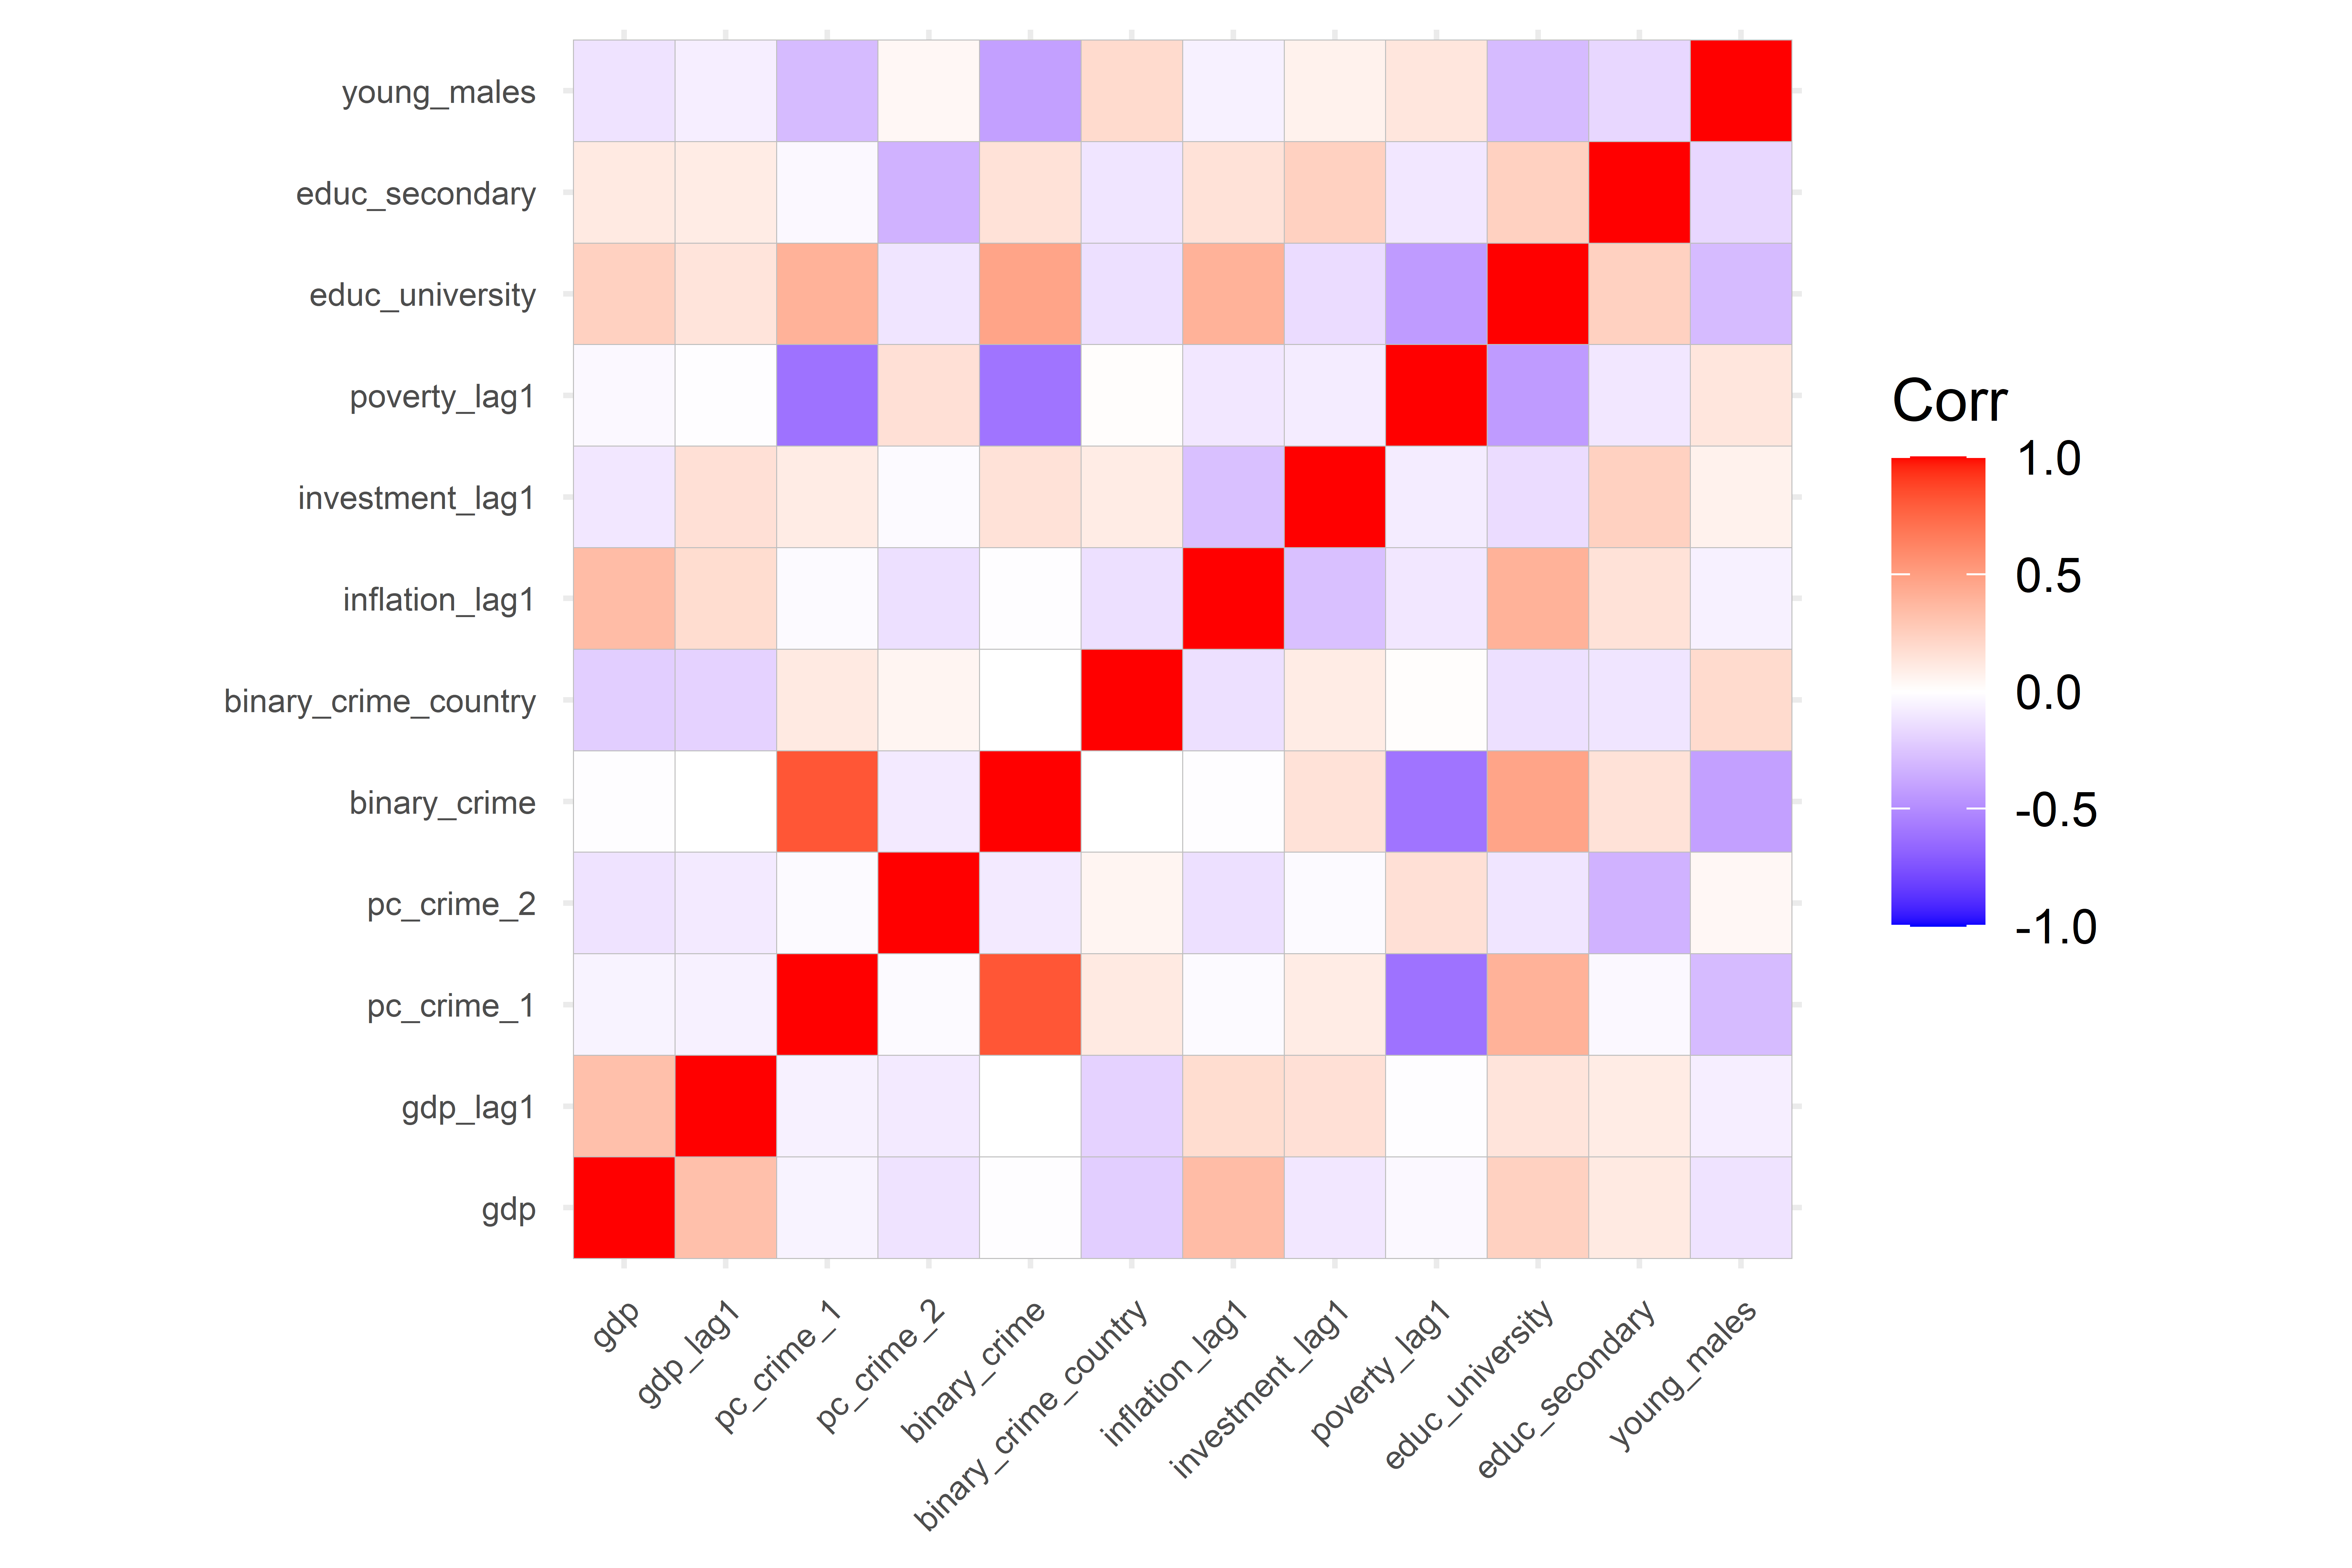
\includegraphics[trim={0 0 0 0},width=\linewidth]{charts/corr_matrix_paper.png}
\begin{flushleft}
\footnotesize{\textit{Note:} This matrix shows correlations between real GDP-growth, crime variables and controls. High absolute correlations indicate relevance of the variable for a potential model.
\label{fig:corr_matrix_paper}	
}
\end{flushleft}
\end{minipage}
\end{figure}

The scatter plot in Figure \ref{fig:scatter_pca} depicts crime data of countries in in only two dimensions using the first two principal components. We can see some clusters of similar crime characteristics for observations. Adding the color scale for GDP-growth, we cannot see a clear dependence between clusters and GDP-growth. \footnote{Categorizing countries similarity based on crime characteristics could be an interesting direct application of this reduction of dimensionality, but is not the aim of this paper.}

Both the descriptive table and correlation matrix show a negative relationship of the "binary crime country" measure and GDP-growth. However, this is only an indication for a causal relationship because effects of other variables are not controlled for.

\section{Results}
\label{Results}


Table \ref{construced_crime_measure} shows regression results for the self-constructed crime measures. "Binary crime" and "binary crime country" coefficients are estimates of the Rubin-causal average treatment effect. 
None of the crime measures is significant. Only "binary crime" has the expected sign and has an economically relevant size (GDP-growth 0.8\% lower with high crime). However, as argued before the crime measure is mostly constant over time and could be correlated with unobserved variables that impact GDP-growth. The measure "binary crime country" estimates that in countries with higher crime than average, GDP-growth is 0.022\% higher than with lower crime than average and is insignificant.
For the control variables, only lagged GDP-growth is significant on a 10 \% level. With an adjusted $R^2$ of 0.58, all models explain a relatively large share of variation in GDP-growth, indicating that the GDP-model itself successfully controls for some variation of GDP due to other factors than crime.

Table \ref{tab:crime_case_number} shows results for the Granger-causal approach similar to \cite{entorf} with all offense categories as regressors. The coefficients are not jointly significant (p-value of 0.14), indicating no significant effect of crime in GDP. 
The results are similar to those of \cite{entorf}, who also do not find a significant effect of crime on GDP-growth. 

One issue of this empirical analysis is the low number of observations combined with a flexible model with $\sim$ 50 regressors due to the fixed effects. This makes it hard to achieve significant results which can e.g. be seen by the low significance of lagged GDP-growth and other controls which are typically regarded as key factors for GDP-modeling. The specification might focus too much on reducing the the bias of the analysis by controlling for many possible confounding variables, and this comes at the cost of a high variance of estimates. Also, reverse causality is not treated well in the specified model. 

Another aspect introducing noise could be the method to construct a suitable crime measure. 
The interpretation of the first principal component as crime index measure is harmed by the different impact of homicide on the crime index. Also, the reduction to a binary measure can lead to a loss in relevant information, which is especially  relevant for only few observations. +


\begin{singlespace}
		\begin{table}[!htbp]
			\centering
			\def\sym#1{\ifmmode^{#1}\else\(^{#1}\)\fi}
			\begin{threeparttable}
				\caption{Regression Results - Constructed Crime Measures}\label{construced_crime_measure} 
\begin{tabular}{@{\extracolsep{5pt}}p{3cm} p{3cm} p{3cm} p{3cm} p{3cm} } 
\\[-1.8ex]\hline 
\hline \\[-1.8ex] 
 & \multicolumn{4}{c}{\textit{Dependent variable: real GDP-growth}} \\ 
\cline{2-4} 
\\Used crime measure & pc crime 1 & pc crime 2 & binary crime & binary crime country\\ 
\hline \\[-1.8ex] 
 crime measure & 0.594 & 0.653 &$-$0.801  & 0.022 \\ 
  & (0.445) & (0.636) & (1.010) &  (0.331) \\ 
  & & & & \\ 
\hline \\[-1.8ex] 
 gdp lag1 & 0.152$^{**}$ & 0.158$^{**}$ & 0.160$^{**}$ & 0.158$^{**}$ \\ 
  & (0.063) & (0.063) & (0.064) & (0.064) \\ 
  & & & & \\ 
 inflation lag1 & $-$0.048 & $-$0.027 & $-$0.041 & $-$0.041 \\ 
  & (0.054) & (0.055) & (0.054) & (0.055) \\ 
  & & & & \\ 
 investment lag1 & $-$0.089 & $-$0.098 & $-$0.095 & $-$0.097 \\ 
  & (0.064) & (0.064) & (0.064) & (0.064) \\ 
  & & & & \\ 
 poverty lag1 & 0.088 & 0.075 & 0.084 & 0.080 \\ 
  & (0.096) & (0.096) & (0.096) & (0.096) \\ 
  & & & & \\ 
 educ university & 0.025 & 0.009 & 0.014 & 0.017 \\ 
  & (0.065) & (0.066) & (0.065) & (0.065) \\ 
  & & & & \\ 
 educ secondary & 0.118 & 0.123 & 0.109 & 0.119 \\ 
  & (0.077) & (0.077) & (0.078) & (0.077) \\ 
  & & & & \\ 
 young males & 0.147 & 0.058 & 0.270 & 0.206 \\ 
  & (0.364) & (0.390) & (0.370) & (0.363) \\ 
  & & & & \\ 
\hline \\[-1.8ex] 
Observations & 269 & 269 & 269 & 269 \\ 
R$^{2}$ & 0.657 & 0.656 & 0.655 & 0.654 \\ 
Adjusted R$^{2}$ & 0.582 & 0.581 & 0.580 & 0.579 \\ 
Residual Std. Error (df = 220) & 2.181 & 2.184 & 2.186 & 2.189 \\ 
F Statistic (df = 48; 220) & 8.774$^{***}$ & 8.730$^{***}$ & 8.704$^{***}$ & 8.667$^{***}$ \\ 
\hline 
\end{tabular}
\begin{footnotesize}
				\begin{tablenotes}
					\item \textit{Note:} 
Standard errors in parentheses. \sym{*} \(p<0.1\), \sym{**} \(p<0.05\), \sym{***} \(p<0.01\). 
Each column shows estimation results for regressing real GDP-growth 
on crime and control variables. Control variables of the previous year are labeled lag1.\\ 
				\end{tablenotes}
			\end{footnotesize}
			\end{threeparttable}
\end{table} 
\end{singlespace}

\section{Conclusion}
\label{Conclusion}
economic cost of crime
Paper: unit costing and macro appraoch

own analysis. Crime index, causal effect, panel data approach, eu countries, no sign effect of crime on gdp growth



Further ideas: longer time frame, more variables and better selection, refine apporach of crime measure, e.g. use constructed crime indices (or compare measure with constructed indices), control for reverse causality 
\& test different time delay effects - VAR model, lots of data
 more model specifications
 
OR: search for more regional effects where impact might be stronger & more variation in crime: e.g. terror attacks on econ activ,  as already done: crime hot spots on house prices
 
\clearpage


\addcontentsline{toc}{section}{Works cited}        % Fuegt im Inhaltsverzeichnis "References" hinzu
\bibliography{literature}   

\newpage

\section*{Appendix}




\begin{figure}
\begin{minipage}{0.9\textwidth}
\captionof{figure}{Crime Principal Components and GDP-growth}
  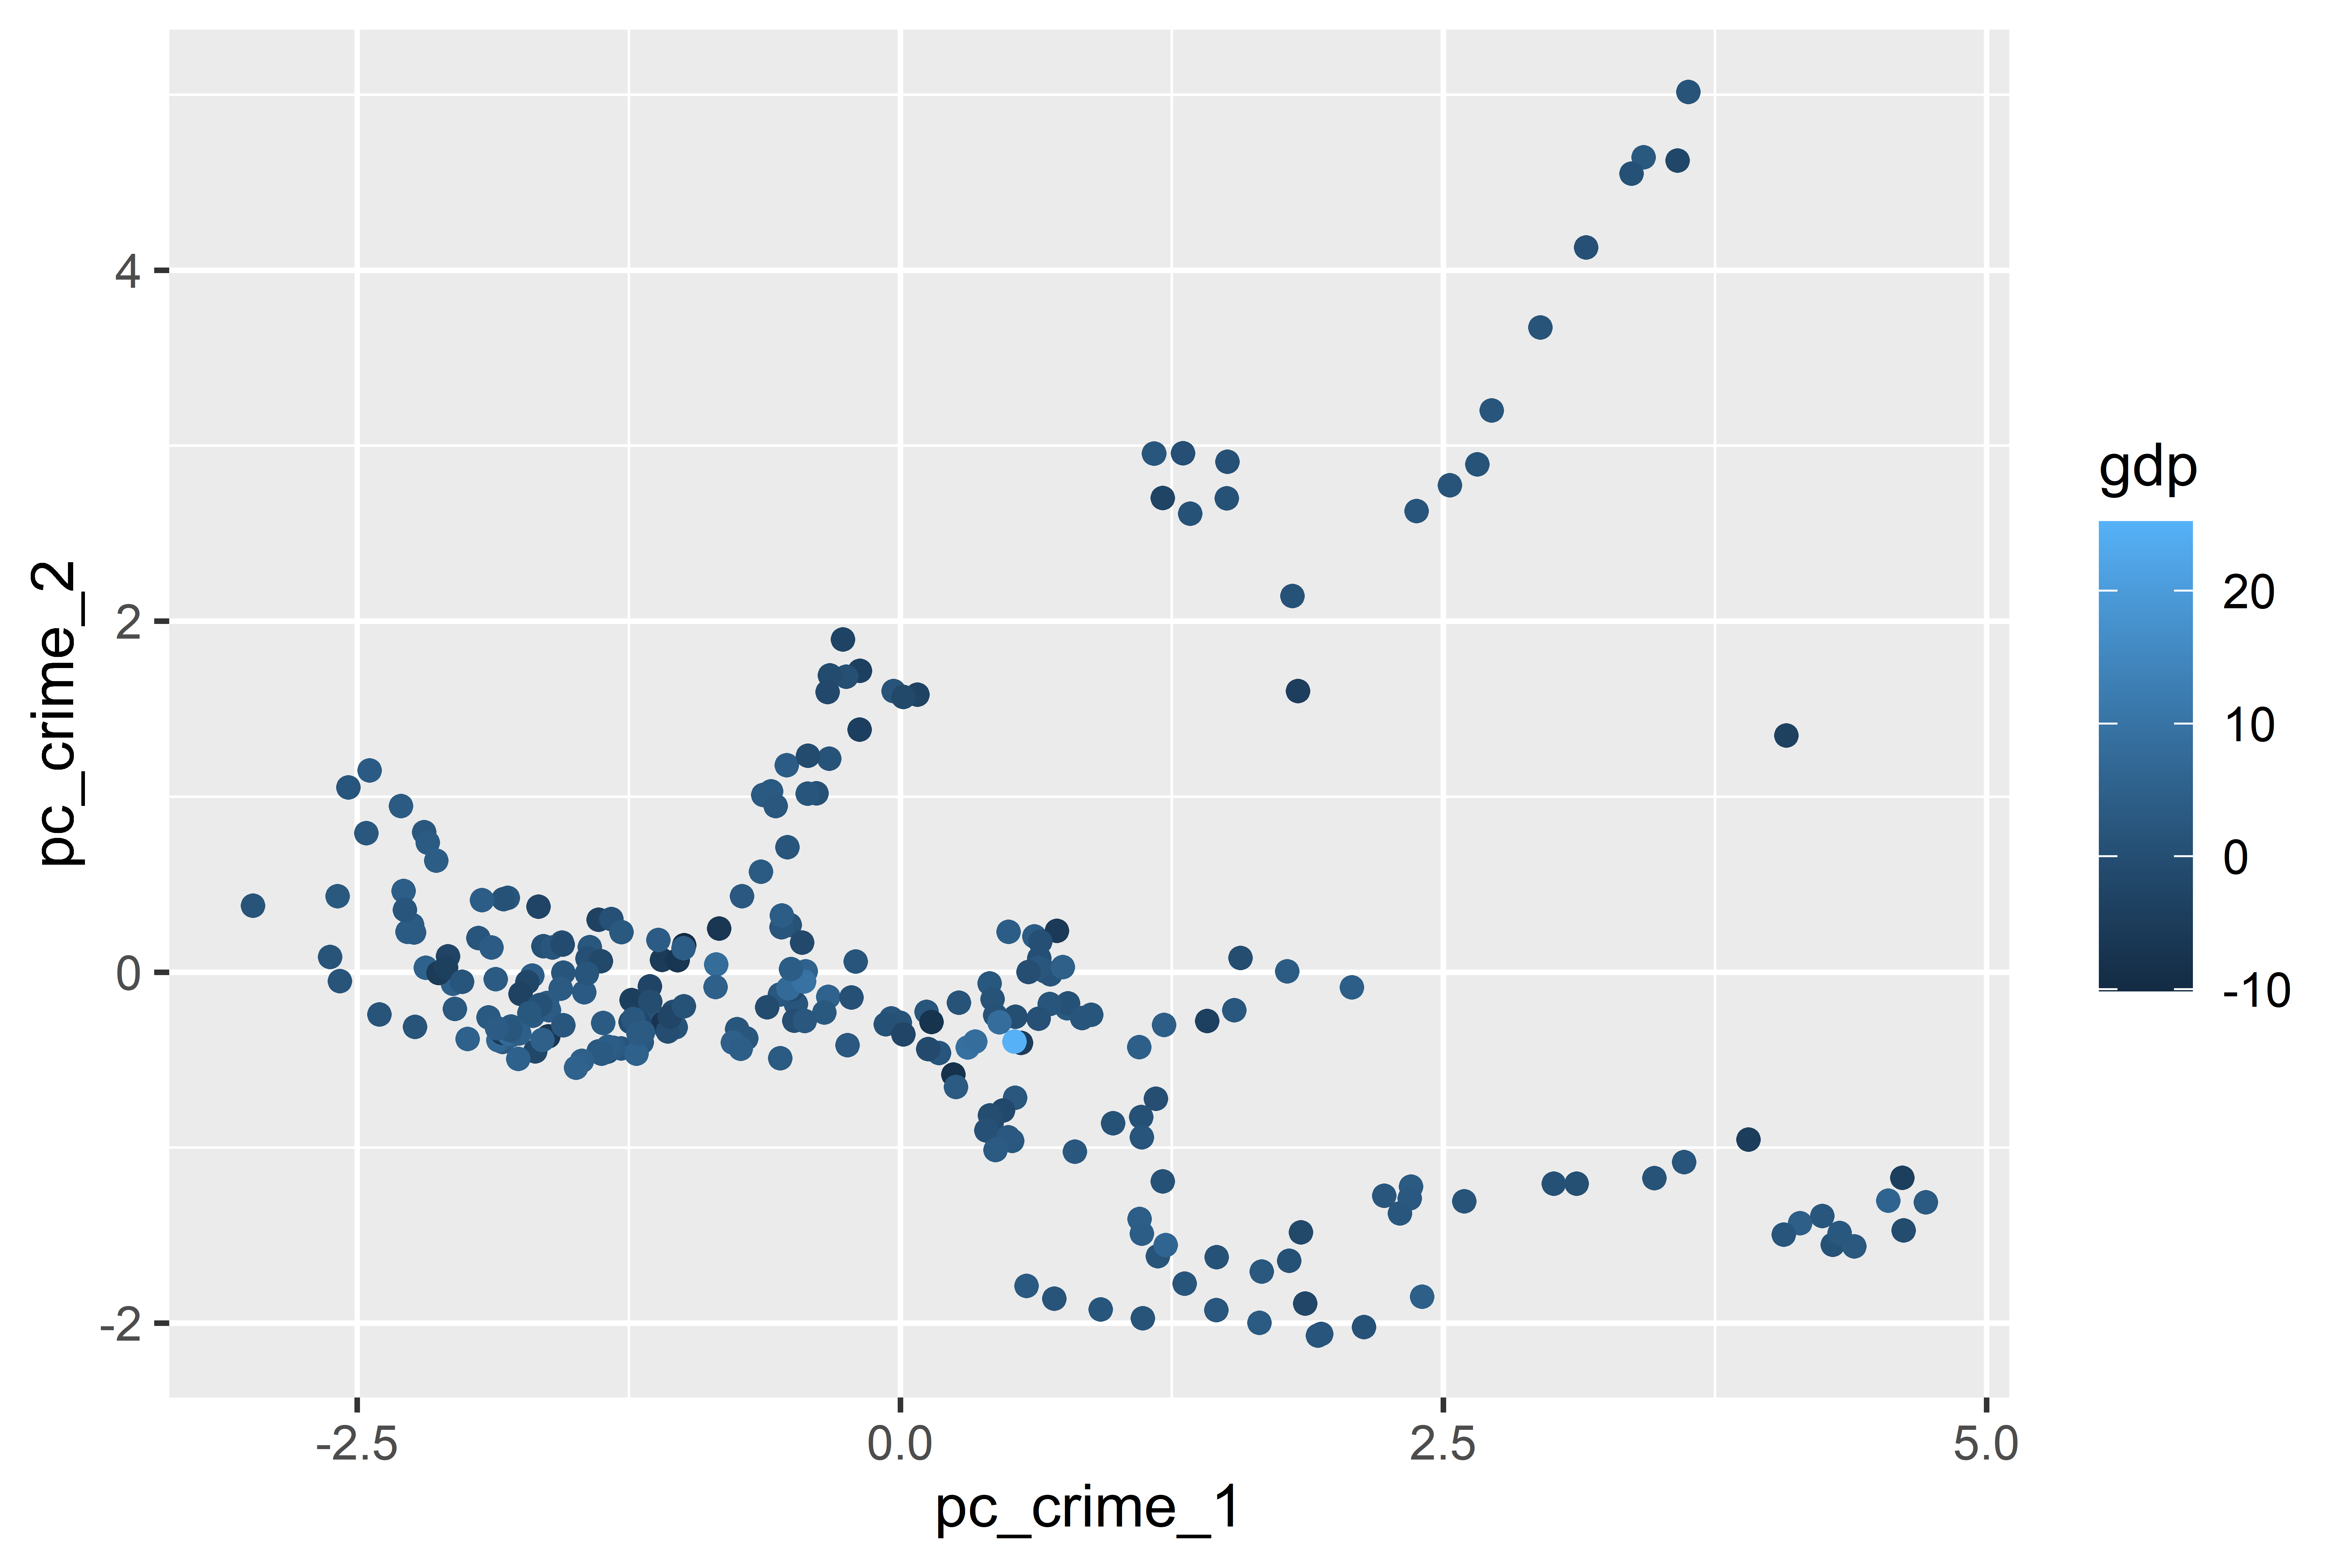
\includegraphics[trim={0 0 0 0},width=\linewidth]{charts/scatter_pca.png}
\begin{flushleft}
\footnotesize{\textit{Note:} This scatter plots depicts the relationship of the first and second crime principal component and real gdp-growth in \%. No clear pattern or clusters can be detected.
\label{fig:scatter_pca}	
}
\end{flushleft}
\end{minipage}
\end{figure}


\begin{figure}

\begin{minipage}{0.45\textwidth}
  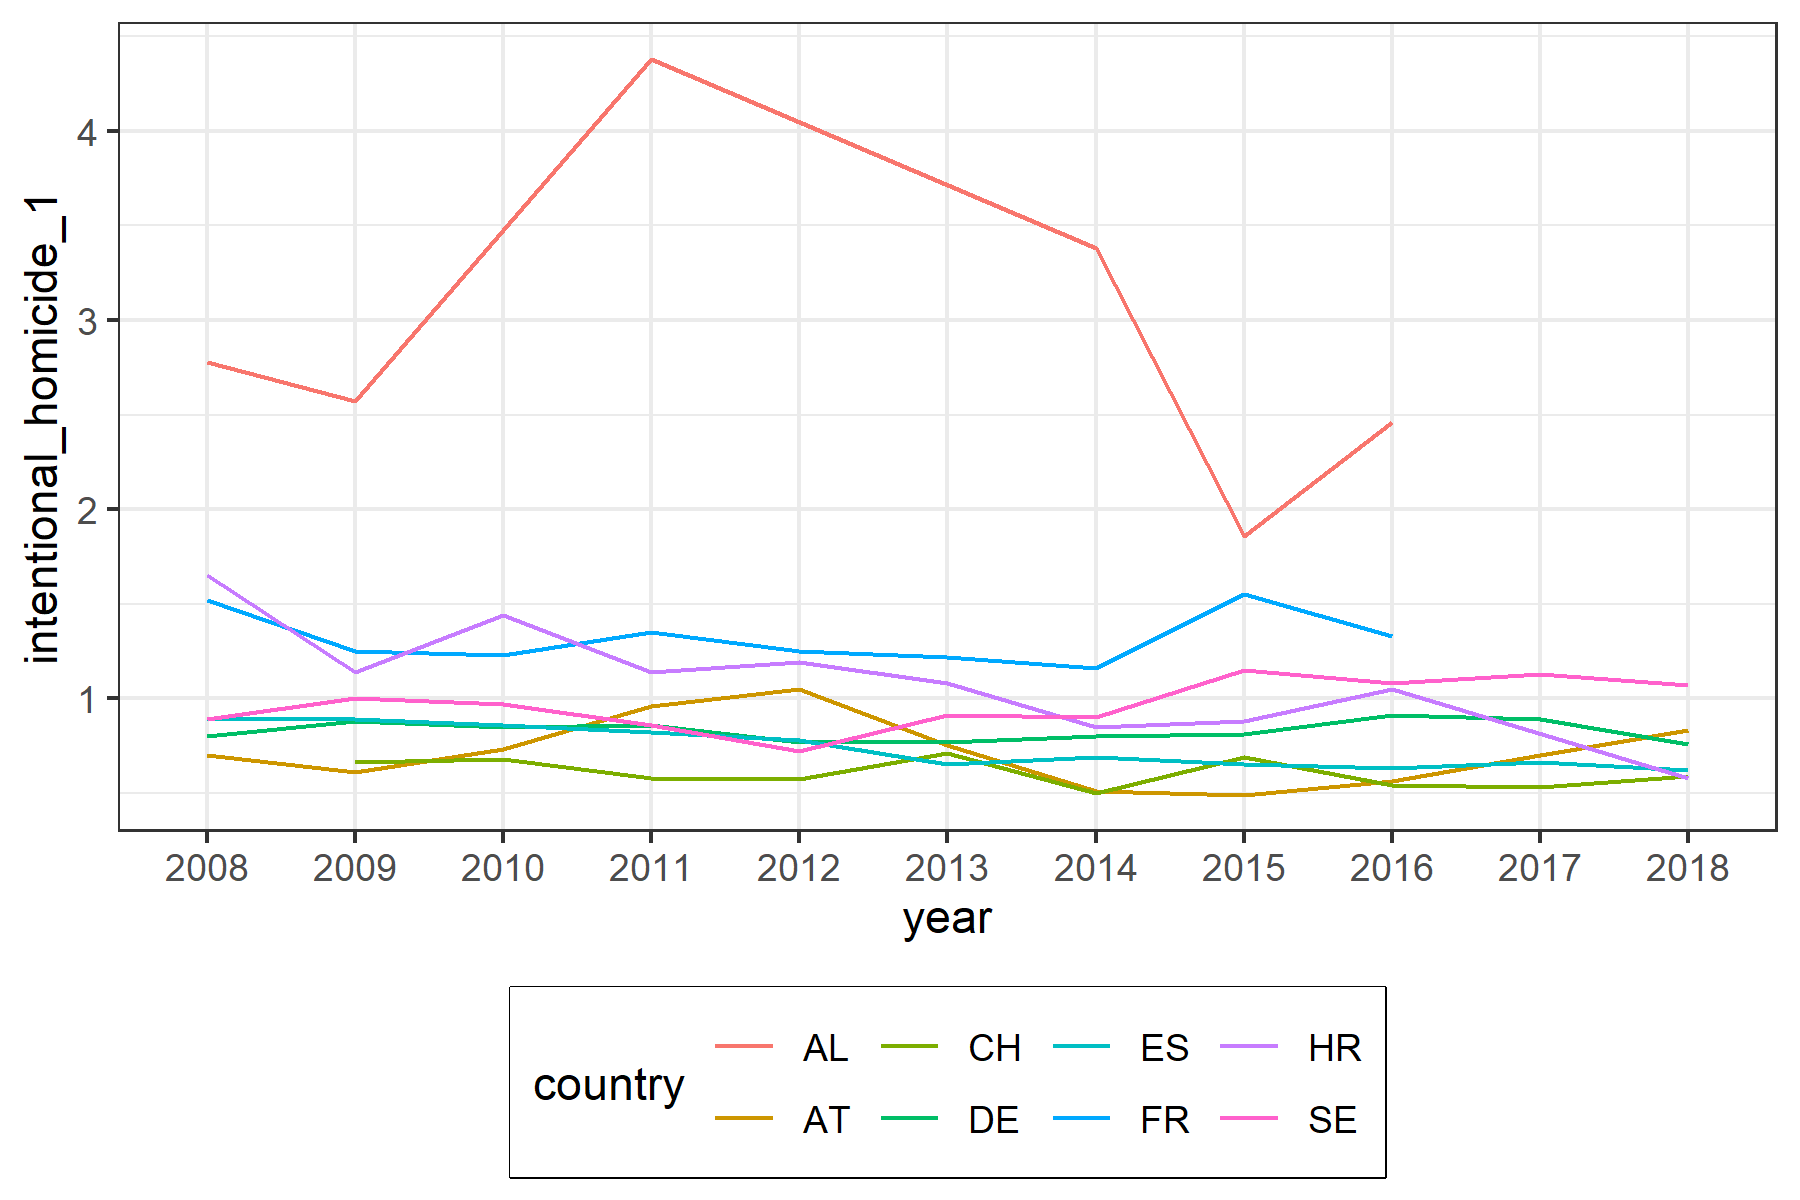
\includegraphics[trim={0 0 0 0},width=\linewidth]{charts/des_line_intentional_homicide_1_.png}
\end{minipage}
\begin{minipage}{0.45\textwidth}
  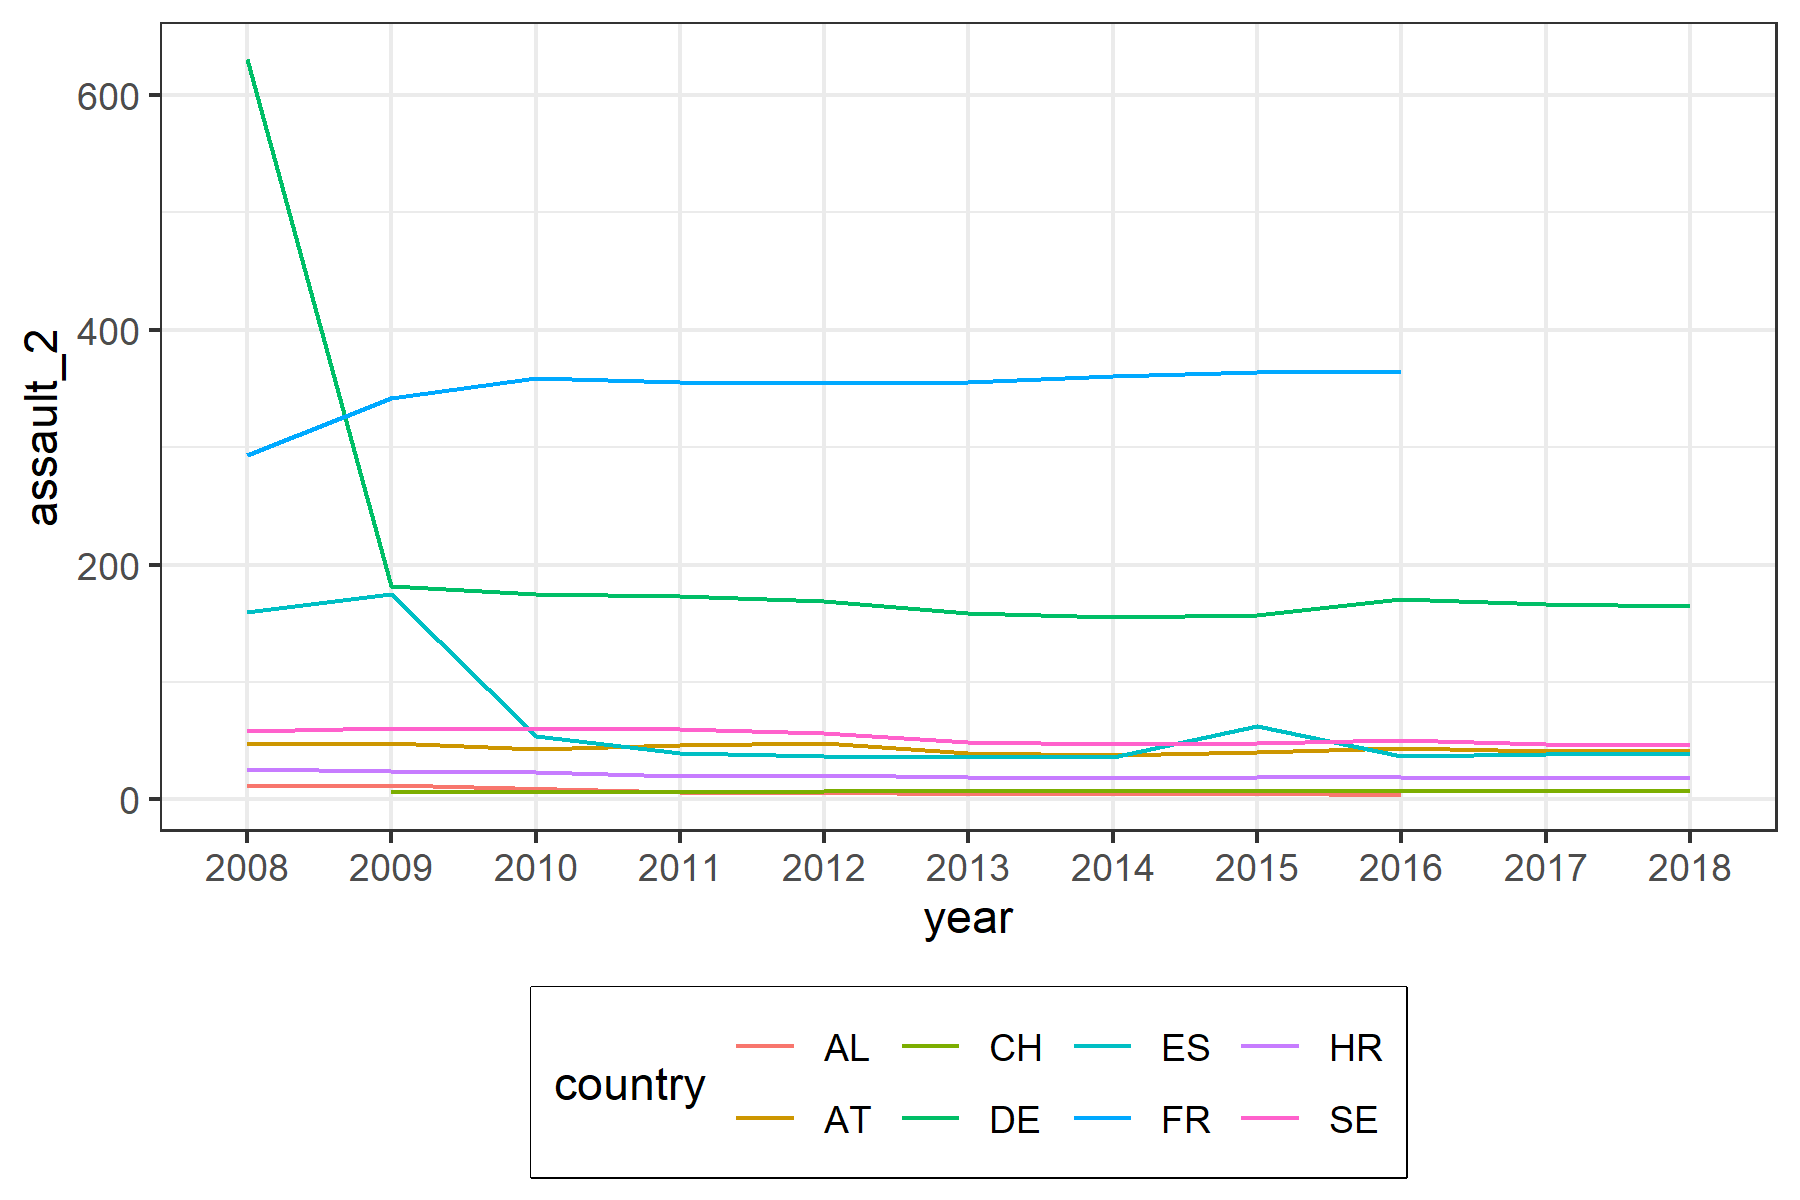
\includegraphics[trim={0 0 0 0},width=\linewidth]{charts/des_line_assault_2_.png}
\end{minipage}
\begin{minipage}{0.45\textwidth}
  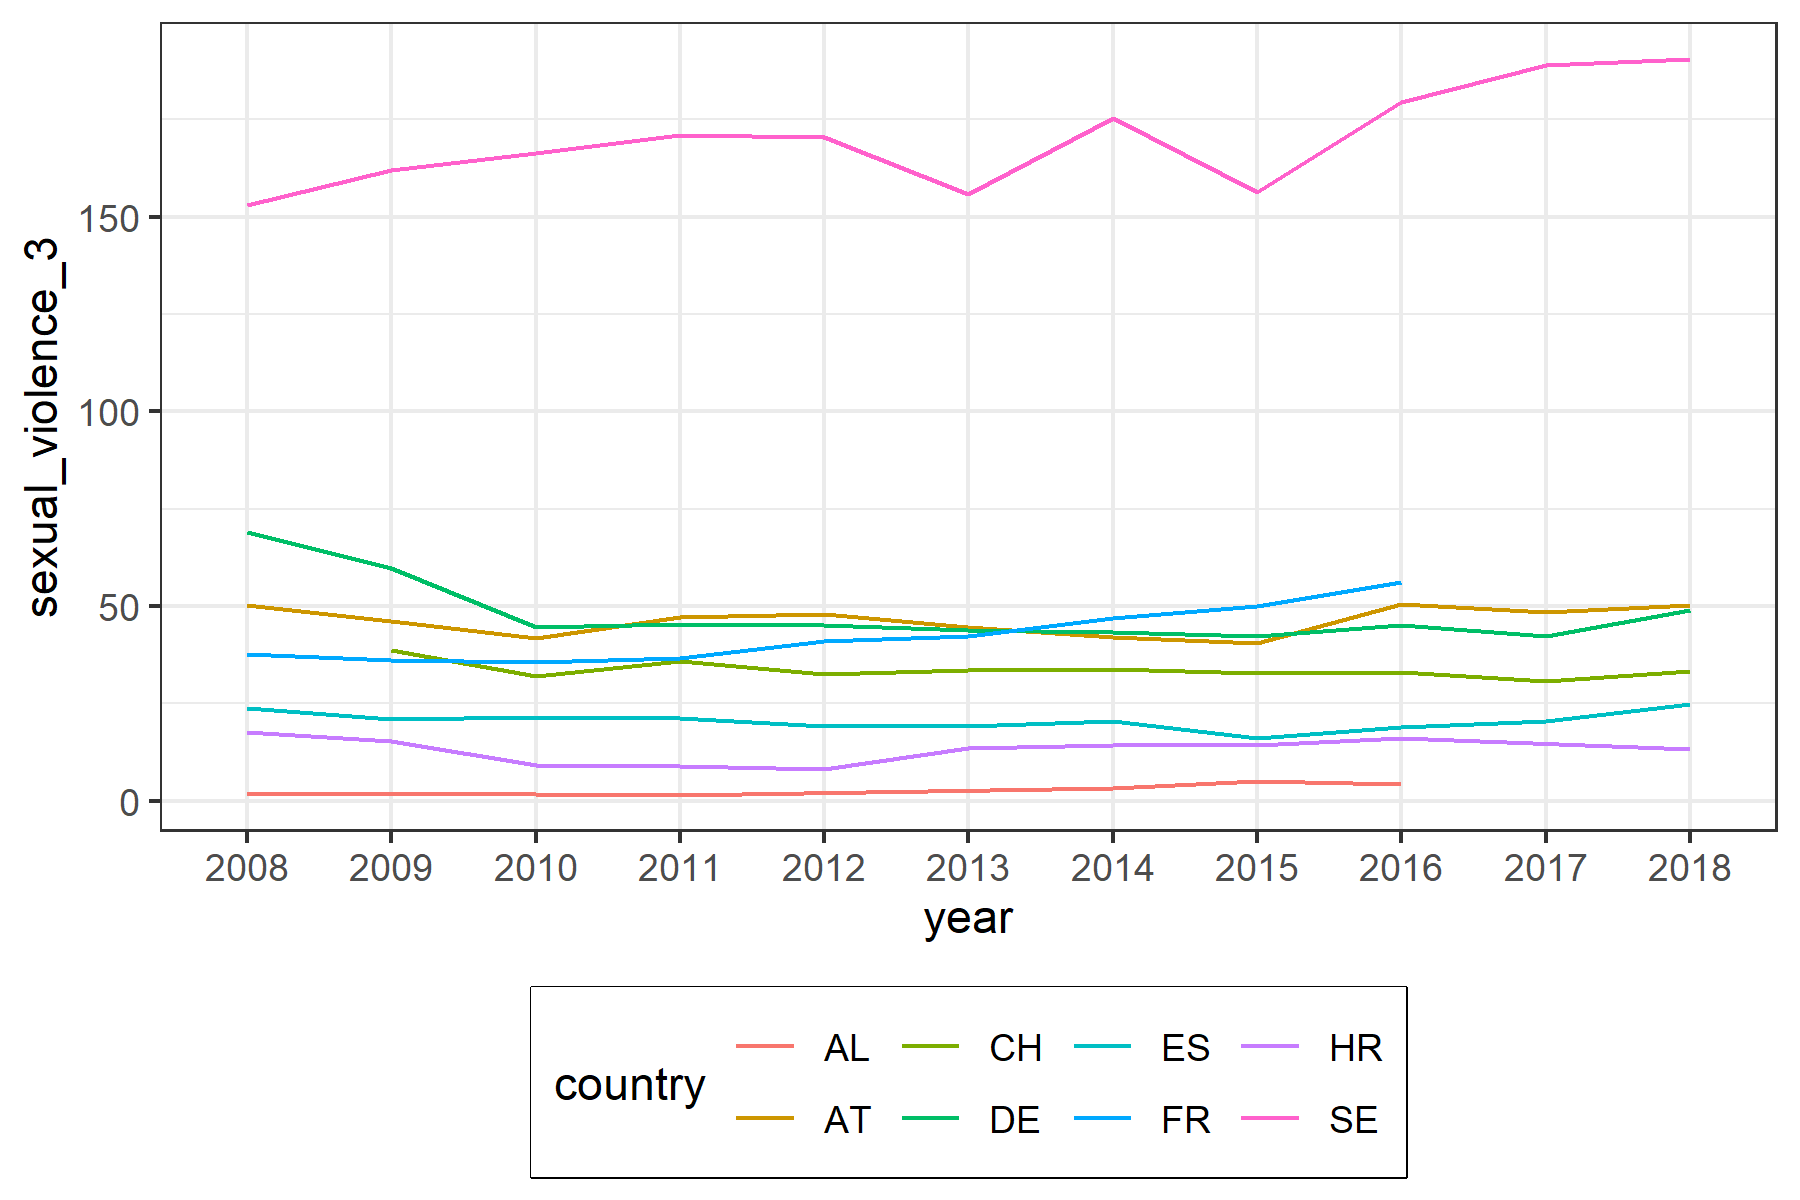
\includegraphics[trim={0 0 0 0},width=\linewidth]{charts/des_line_sexual_violence_3_.png}
\end{minipage}
\begin{minipage}{0.45\textwidth}
  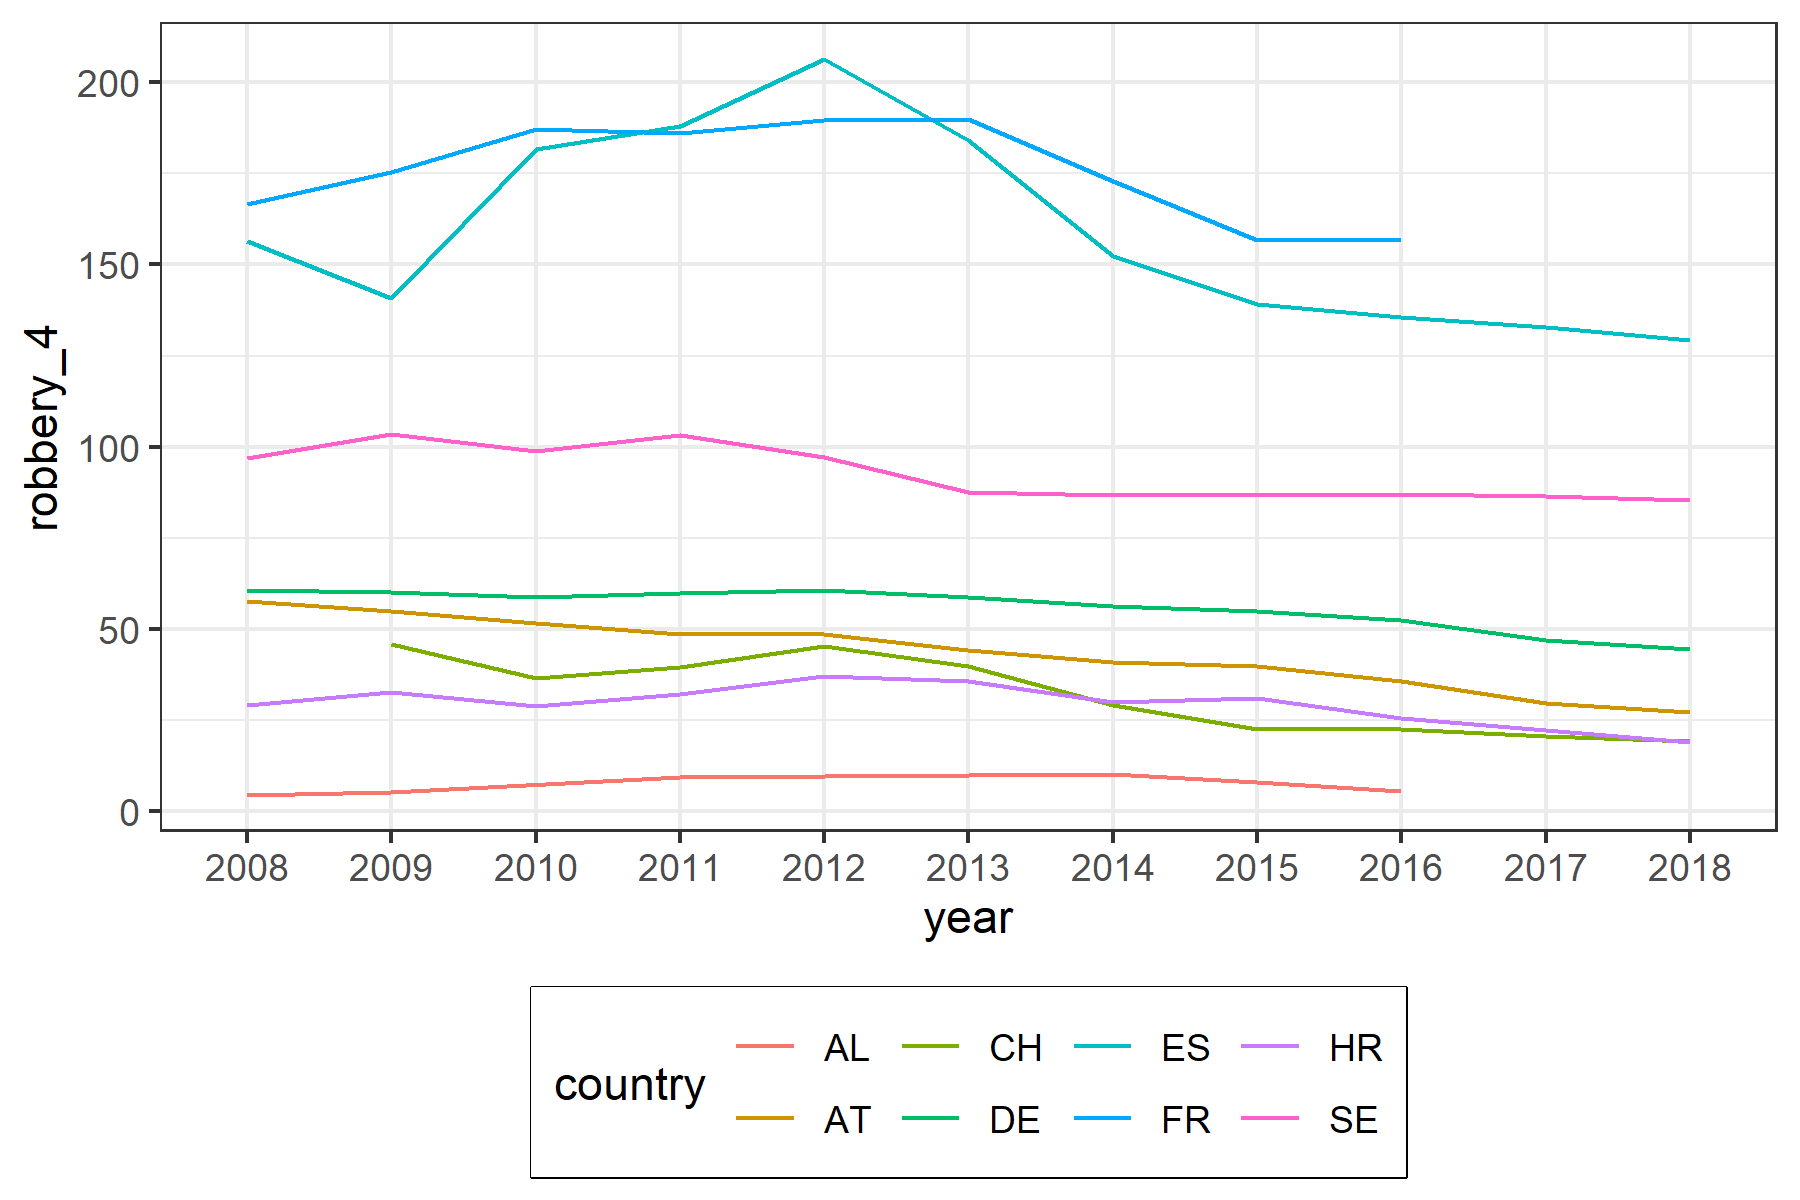
\includegraphics[trim={0 0 0 0},width=\linewidth]{charts/des_line_sexual_robbery_4_.png}
\end{minipage}
\begin{minipage}{0.45\textwidth}
  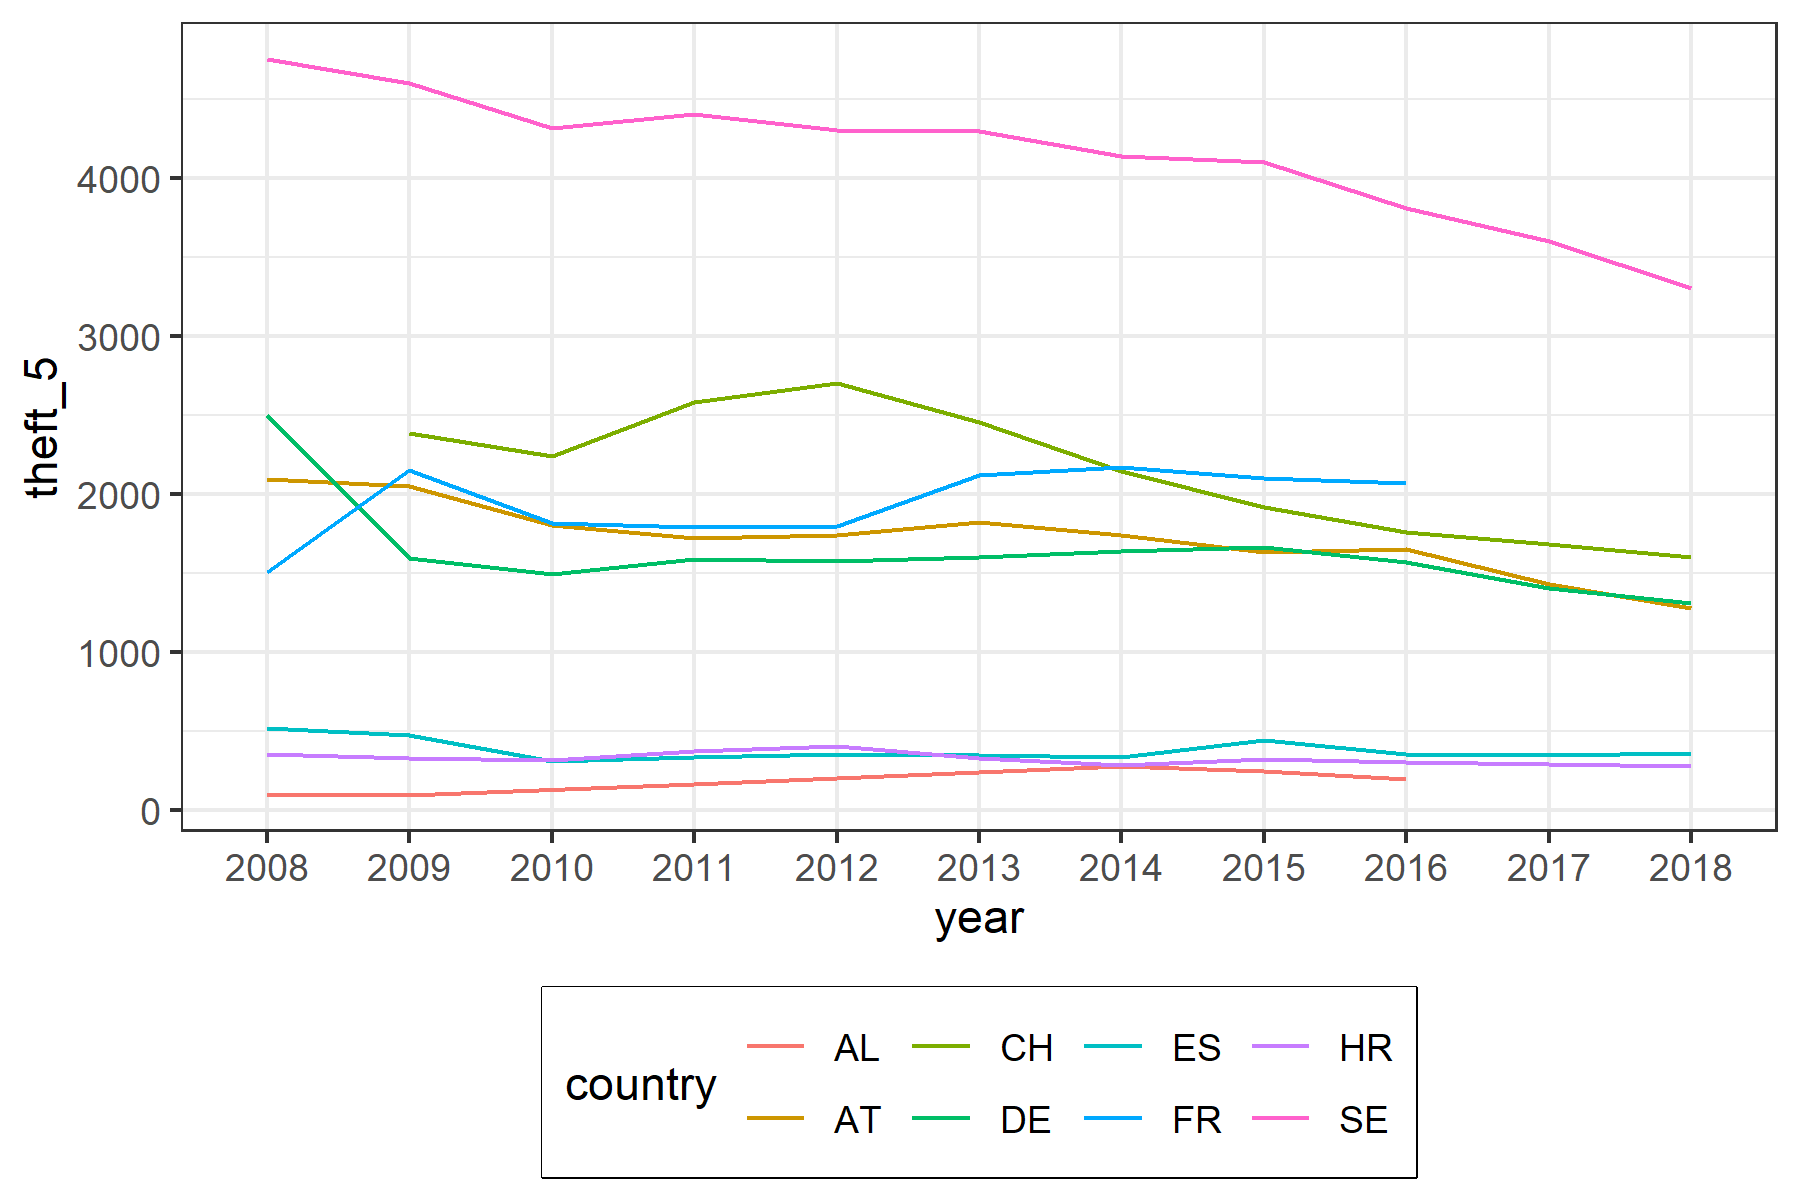
\includegraphics[trim={0 0 0 0},width=\linewidth]{charts/des_line_theft_5_.png}
\end{minipage}
\begin{minipage}{0.45\textwidth}
  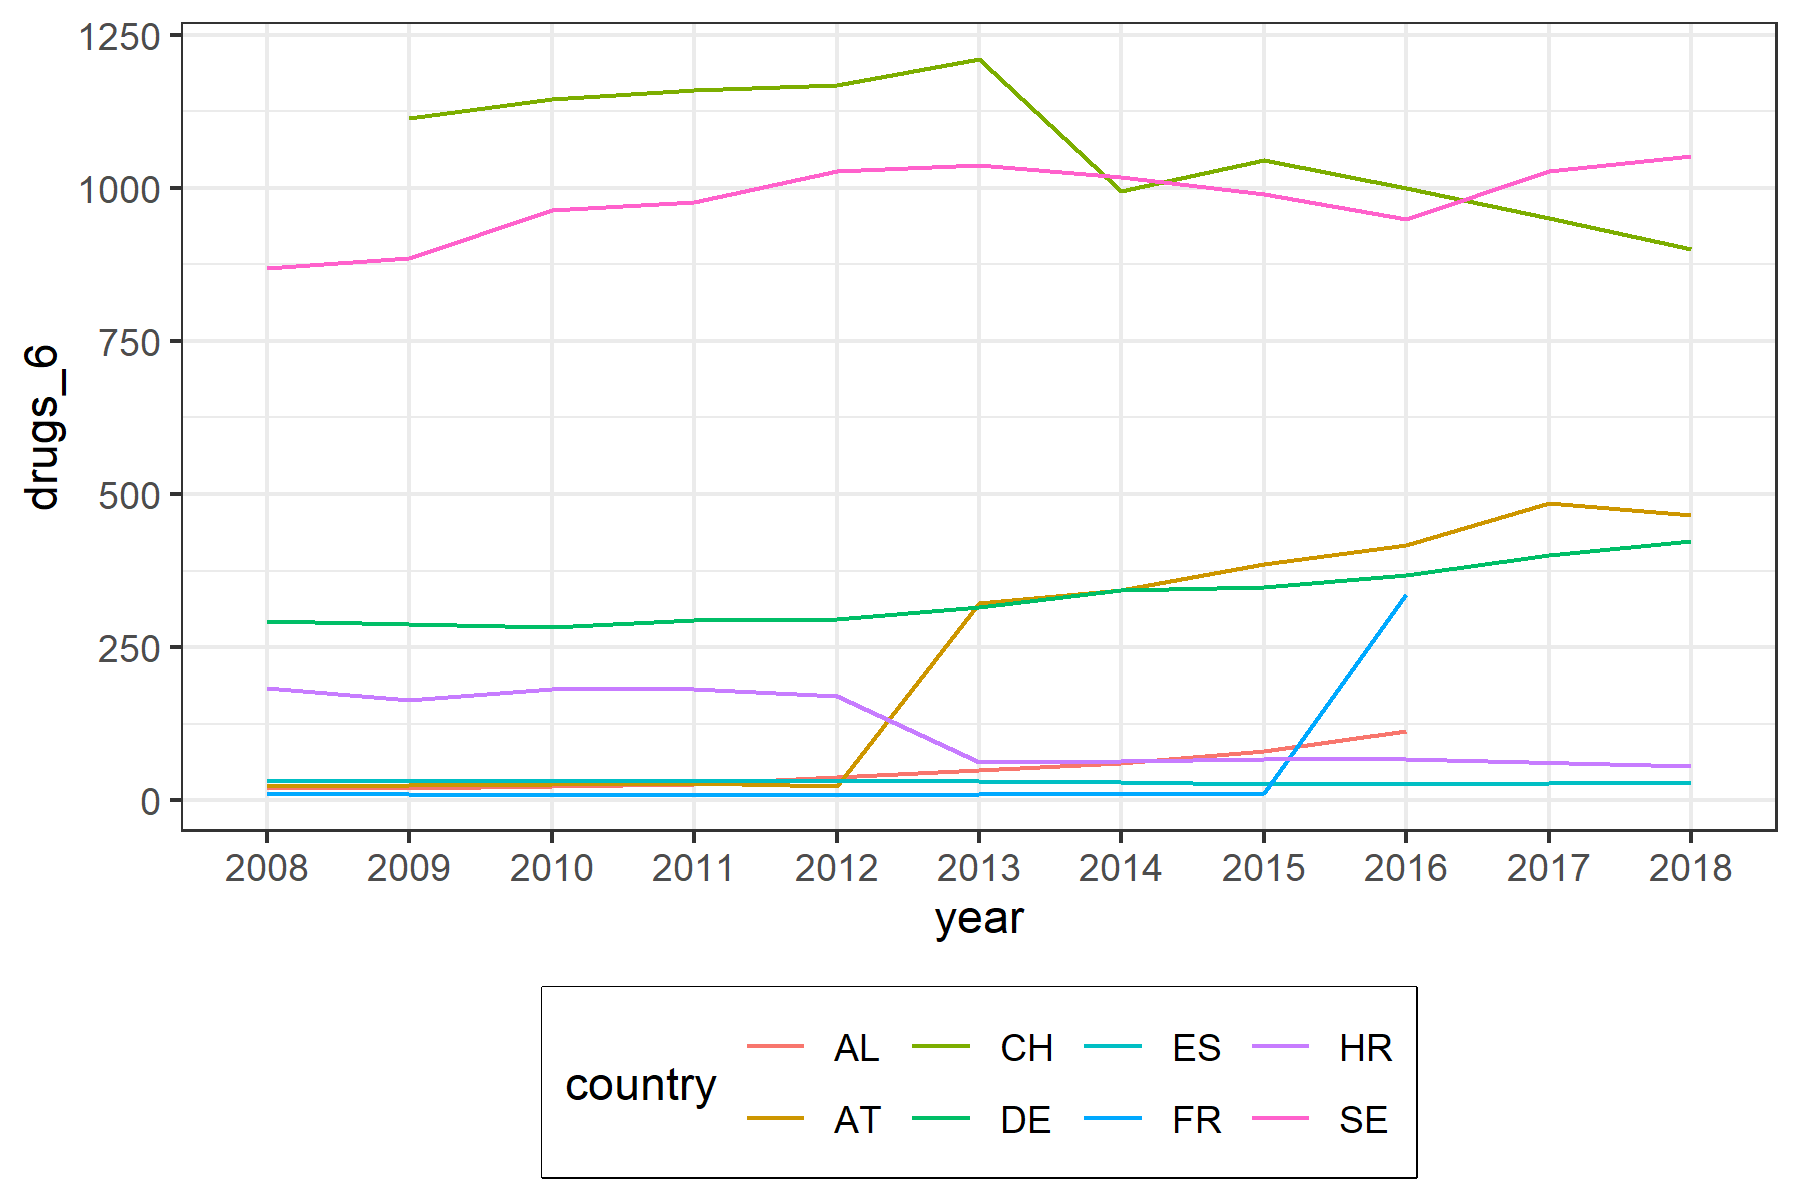
\includegraphics[trim={0 0 0 0},width=\linewidth]{charts/des_line_drugs_6_.png}
\end{minipage}

\begin{flushleft}
\captionof{figure}{Crime case data by offense type - selected countries}
\footnotesize{\textit{Note:} This figure shows the reported case numbers for different offense categories for selected European countries.
\label{fig:crime_case_data}	
}
\end{flushleft}
\end{figure}


\begin{figure}
\begin{minipage}{0.9\textwidth}
\captionof{figure}{Crime principal component 1 - selected countries}
  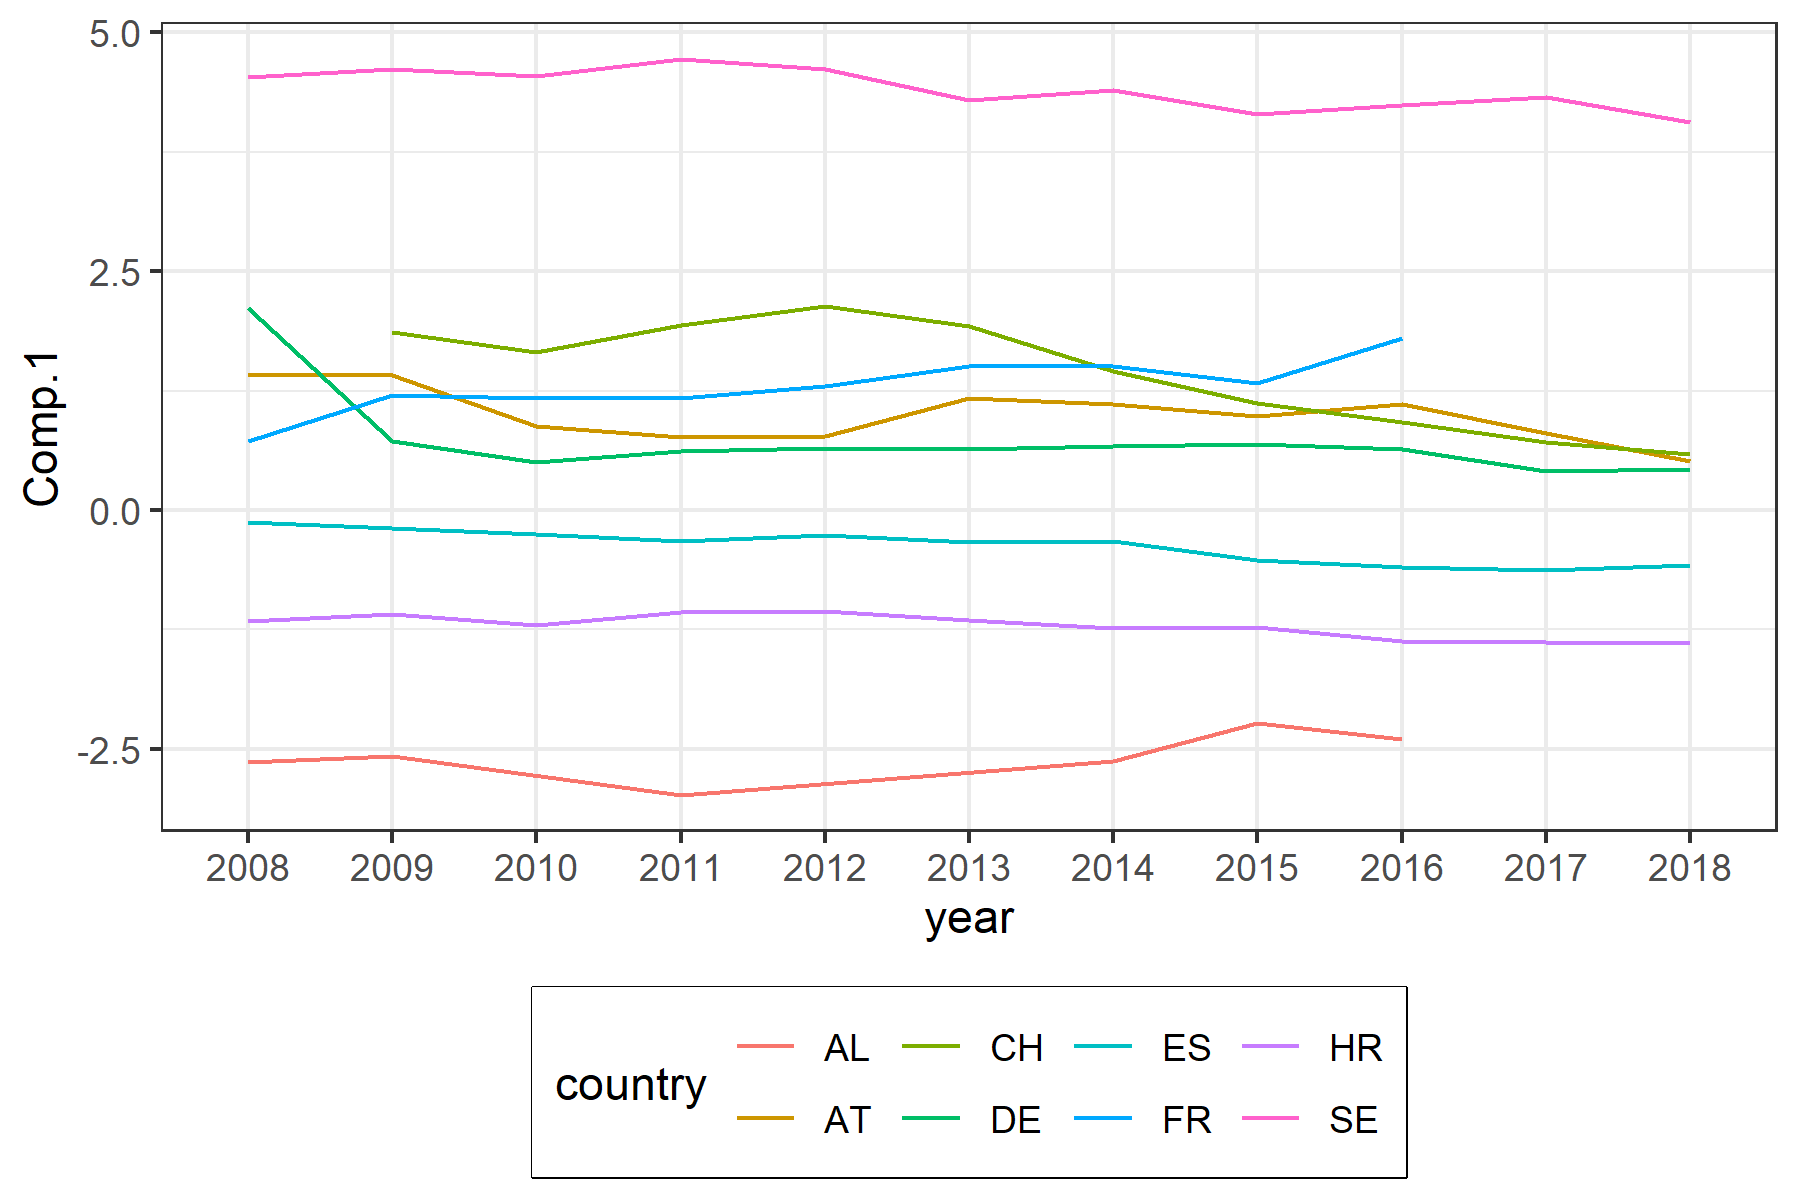
\includegraphics[trim={0 0 0 0},width=\linewidth]{charts/princial_component_1.png}
\begin{flushleft}
\footnotesize{\textit{Note:} This chart depicts the first crime principal component over time for different countries. 
\label{fig:princial_component_1}	
}
\end{flushleft}
\end{minipage}
\end{figure}



\begin{singlespace}
		\begin{table}[!htbp]
			\centering
			\def\sym#1{\ifmmode^{#1}\else\(^{#1}\)\fi}
			\begin{threeparttable}
				\caption{Regression Results - Crime Case Numbers}\label{tab:crime_case_number} 
\begin{tabular}{@{\extracolsep{5pt}}lc} 
\\[-1.8ex]\hline 
\hline \\[-1.8ex] 
 & \multicolumn{1}{c}{\textit{Dependent variable: real GDP-growth}} \\ 
\cline{2-2}  
\hline \\[-1.8ex] 
 intentional homicide 1 & $-$0.147 \\ 
  & (0.388) \\ 
  & \\ 
  [-1.8ex]
 assault 2 & $-$0.002 \\ 
  & (0.005) \\ 
  & \\ 
  [-1.8ex]
 sexual violence 3 & 0.029$^{*}$ \\ 
  & (0.017) \\ 
  & \\ 
  [-1.8ex]
 robbery 4 & 0.005 \\ 
  & (0.016) \\ 
  & \\ 
  [-1.8ex]
 burglary 5 & $-$0.002 \\ 
  & (0.002) \\ 
  & \\
  [-1.8ex]
 theft 5 & 0.002$^{*}$ \\ 
  & (0.001) \\ 
  & \\ 
 drugs 6 & $-$0.004$^{**}$ \\ 
  & (0.002) \\ 
    [-1.8ex]
  & \\
  \hline
 gdp lag1 & 0.121$^{*}$ \\ 
  & (0.064) \\ 
  & \\ 
  [-1.8ex]
 inflation lag1 & $-$0.014 \\ 
  & (0.056) \\ 
  & \\ 
  [-1.8ex]
 investment lag1 & $-$0.068 \\ 
  & (0.067) \\ 
  & \\ 
  [-1.8ex]
 poverty lag1 & 0.064 \\ 
  & (0.098) \\ 
  & \\ 
  [-1.8ex]
 educ university & 0.027 \\ 
  & (0.068) \\ 
  & \\ 
  [-1.8ex]
 educ secondary & 0.108 \\ 
  & (0.081) \\ 
  & \\ 
  [-1.8ex]
 young males & 0.043 \\ 
  & (0.406) \\ 
  & \\ 
  [-1.8ex]
\hline \\[-1.8ex] 
Observations & 269 \\ 
R$^{2}$ & 0.671 \\ 
Adjusted R$^{2}$ & 0.588 \\ 
Residual Std. Error & 2.165 (df = 214) \\ 
F Statistic & 8.088$^{***}$ (df = 54; 214) \\ 
\hline \\[-1.8ex] 
Test Joint Significance Crime Cases & p-val: 0.14 \\ 
\hline 
\end{tabular}
\begin{footnotesize}
				\begin{tablenotes}
					\item \textit{Note:} 
Standard errors in parentheses. \sym{*} \(p<0.1\), \sym{**} \(p<0.05\), \sym{***} \(p<0.01\). 
The column shows the results of regressing real GDP-growth on crime and control variables using the raw case numbers for different offense types as crime measures. Control variables of the previous year are labeled lag1.\\ 
				\end{tablenotes}
			\end{footnotesize}
			\end{threeparttable}
\end{table} 
\end{singlespace}

\end{document}